\documentclass[12pt,oneside]{report}
\usepackage[T1]{fontenc}		% Einstellungen fuer Umlaute usw.
\usepackage[utf8x]{inputenc}
\usepackage[ngerman]{babel}

\usepackage{parskip}			% Einstellungen fuer Absaetze: Abstand statt Einrueckung

\usepackage[a4paper,			% Papierformat A4
	    left=2.5cm,				% linker Rand
	    right=2.5cm,			% rechter Rand
	    top=1.5cm,				% oberer Rand
	    bottom=1.5cm,			% unter Rand
	    marginparsep=5mm,		% Abstand der Randnotizen
	    marginparwidth=10mm, 	% Breite der Randnotizen
	    headheight=7mm,			% Hoehe der Kopfzeile
	    headsep=1.2cm,			% Abstand der Kopfzeile
	    footskip=1.5cm,			% Abstand der Fusszeile
	    includeheadfoot]{geometry}

\usepackage{fancyhdr}						% Konfiguration von Kopf- und Fusszeilen
\pagestyle{fancy}							% Seitenstil 'fancy'
\fancyhf{}									% vorhandene Einstellungen loeschen
\setlength{\headwidth}{\textwidth}			% Kopf- und Fusszeile so breit wie der Haupttext
\fancyfoot[R]{\thepage} 					% Festlegung des Seitenstils: Seitenzahlen in der Fusszeile rechts
\fancyfoot[L]{\leftmark}					% Kapitelnr. und -Bezeichnung in der Fusszeile links
\fancyhead[R]{\IhreArbeit}					% "Bachelorarbeit" in der Kopfzeile rechts
\renewcommand{\chaptermark}[1]{			% Definition der Ausgabe des Kapitels
  \markboth{Kapitel \thechapter. #1}{}}
\renewcommand{\headrulewidth}{0.5pt}		% Trennlinie zwischen Kopfzeile und Haupttext
\renewcommand{\footrulewidth}{0.5pt}		% Trennlinie zwischen Haupttext und Fusszeile
\fancypagestyle{plain}{					% Anpassung des Seitenstils 'plain' bei Beginn neuer Kapitel
  \fancyhf{}								% Vorbelegung loeschen
  \fancyfoot[C]{\thepage}					% Seitenzeilen in der Fusszeile mittig
  \fancyhead[R]{\IhreArbeit}				% "Bachelorarbeit" in der Kopfzeile rechts
}

\usepackage{amsmath}			% Pakete fuer den Mathematikmodus
\usepackage{amssymb}
\usepackage[intlimits]{empheq}

\usepackage[sc]{mathpazo}		% Schriftart Palatino fuer Haupttext und Mathematikmodus
\usepackage{pifont}				% zusaetzliche Symbole

\usepackage[format=hang,		% Einstellung fuer Bildunterschriften
            font={footnotesize},
            labelfont={bf},
            margin=1cm,
            aboveskip=5pt,
            position=bottom]{caption}

\usepackage{graphicx}							% Einbinden von Graphiken
\usepackage[svgnames,cmyk,table,hyperref]{xcolor} 	% Verwendung von Farben
\usepackage{tikz}								% Erstellen von Grafiken
\usetikzlibrary{positioning,arrows,plotmarks} % 

% 
% Weitere Pakete
%
\usepackage{listings}			% Darstellung von Quellcode
\lstset{
  language=C++,                   % C++ als Sprache
  basicstyle=\ttfamily,           % Schriftart
  keywordstyle=\color{blue},      % Farbe für keywords
  % stringstyle=\color{red},
  frame=single,                         % adds a frame around the code
  framesep=8pt,                         % adds padding between the frame and the code
  commentstyle=\color{green},     % Farbe für comments
  identifierstyle=\color{olive},  % Farbe für Funktionen
}
\usepackage{paralist}			% Darstellung von Listen
\usepackage{float}

\usepackage{microtype,relsize}					% Wird verwendet, um Nachnamen auf Titelseite gesperrt darzustellen
\newcommand*{\Sperren}[1]{\textls*[100]{#1}}

% 
% Persoenliche Angaben
% 
\newcommand*{\Name}{Berkay}
\newcommand*{\Nachname}{Yurdagül}
\newcommand*{\Namezwei}{Manuel}
\newcommand*{\Nachnamezwei}{Pickl}
\newcommand*{\IhrStudiengang}{Medieninformatik}
\newcommand*{\IhrFach}{Physical Computing}
\newcommand*{\IhreArbeit}{Wire \& Warriors}
\newcommand*{\IhrBearbeitungszeitraumVON}{26. April 2023}
\newcommand*{\IhrBearbeitungszeitraumBIS}{14. März 2024}
\newcommand*{\IhrErstpruefer}{Prof. Dipl.-Des. Martin Frey}
\newcommand*{\IhrZweitpruefer}{Prof. Dr.-Ing. Ulrich Schäfer}
\newcommand*{\IhrDrittpruefer}{Prof. Dr.-Ing. Gerald Pirkl}
\newcommand*{\IhreZusammenfassung}{%
Lorem ipsum dolor sit amet, consetetur sadipscing elitr, sed diam nonumy eirmod tempor invidunt ut labore et dolore magna aliquyam erat, sed diam voluptua. At vero eos et accusam et justo duo dolores et ea rebum. Stet clita kasd gubergren, no sea takimata sanctus est Lorem ipsum dolor sit amet. Lorem ipsum dolor sit amet, consetetur sadipscing elitr, sed diam nonumy eirmod tempor invidunt ut labore et dolore magna aliquyam erat, sed diam voluptua. At vero eos et accusam et justo duo dolores et ea rebum. Stet clita kasd gubergren, no sea takimata sanctus est Lorem ipsum dolor sit amet.
}
\newcommand*{\IhreSchluesselwoerter}{test}


\usepackage[bookmarks, raiselinks, pageanchor, % PDF-Einstellungen
            hyperindex, colorlinks,
            citecolor=black, linkcolor=black,
            urlcolor=black, filecolor=black,
            menucolor=black]{hyperref}
\hypersetup{pdftitle={\IhreArbeit},%
            pdfauthor={\Name\ \Nachname \Namezwei \Nachnamezwei},%
            pdfsubject={\IhrFach},%
            pdfkeywords={\IhreSchluesselwoerter}}

%
% Beginn des Textteils
%
\begin{document}
  \pagenumbering{roman}
  \begin{center}
    \Large
    Ostbayerische Technische Hochschule Amberg-Weiden\\
    Fakultät Elektrotechnik, Medien und Informatik\\[1cm]
    Studiengang \IhrStudiengang\\[1cm]
    \IhrFach\\[1cm]
    Projekt \textbf{\IhreArbeit}\\[1cm]
    von\\[1cm]
    \Name\ \Sperren{\textbf{\Nachname}}\\[1cm]
    \Namezwei\ \Sperren{\textbf{\Nachnamezwei}}\\[1cm]
  \end{center}
  \vspace*{4cm}
  \begin{tabbing}
    \underbar{Bearbeitungszeitraum:}\qquad\= von\qquad\=\IhrBearbeitungszeitraumVON\\
                                          \> bis      \>\IhrBearbeitungszeitraumBIS
  \end{tabbing}
  \vspace*{1cm}
  \underbar{1. Prüfer:}\qquad\IhrErstpruefer\par
  \underbar{2. Prüfer:}\qquad\IhrZweitpruefer\par 
  \underbar{3. Prüfer:}\qquad\IhrDrittpruefer
  \clearpage
  \include{formblatt_selbststaendigkeitserklaerung}		% 3. Seite: Formblatt Bestaetigung nach Paragraph 12 APO
  \include{formblatt_summary}			% 4. Seite: Formblatt Zusammenfassung
  \tableofcontents
  \newpage
  \chapter*{Symbole, Formelzeichen und Einheiten}
  \newpage
  \pagenumbering{arabic}
  \chapter{Einführung und Idee}

Das Spiel `Wire \& Warriors' ist ein innovative Spiel, dass die Intensität eines Escape Rooms mit der Geschicklichkeit eines `Heißen Draht'-Spieles vereint. Dieses Spiel stellt eine neue Herangehensweise an das klassiche Konzept dar, indem es Teamarbeit und Geschicklichkeit miteinander verbindert.

\section{Spielkonzept eines Escape-Room}

Ein Escape-Room basiert auf dem Prinzip der Live-Action-Rätselspiele, bei denen Spieler in einem speziell gestalteten Raum oder einer Umgebung eingeschlossen sind. In diesem Raum müssen verschiedene Rätsel gelöst werden, um zu entkommen. Im folgenden werden die Schlüsselkomponenten aufgelistet:

\begin{compactitem}
 \item \textbf{Thematische Umgebung}: Ein Escape-Room besitzt ein Thema und zusätzlich eine Geschichte. Das Thema sowie die Geschichte bilden den Rahmen für die Rästel und Aufgaben.
 \item \textbf{Rätsel und Aufgaben}: Die Spieler im Escape-Room müssen eine Reihe von Rätseln lösen, um zu entkommen. Die Rästel bzw. Aufgaben können aus Beobachtungsaufgaben, Geschicklichkeit oder auch Teamarbeit bestehen. Häufig sind die Rästel thematisch in die Umgebung eingebettet und tragen zur Gesamtgeschichte bei.
 \item \textbf{Zeitlimit}: Die Spieler haben eine festgelegte Zeit (oftmals eine Stunde), um alle Aufgaben zu lösen und aus dem Raum zu entkommen. Dadurch soll Druck erzeugt werden und die Spannung des Spiels erhöhen.
 \item \textbf{Teamarbeit}: Escape-Rooms sind oft auf Teamarbeit ausgelegt, um gemeinsam zu rästeln und zu entkommen.
 \item \textbf{Interaktive Elemente}: Escape-Rooms nutzen technologische und mechanische Vorrichtungen, um das Spielerlebnis zu bereichern.
\end{compactitem}

\section{Spielkonzept vom Heißen Draht-Spiel}
Das Heiße Draht-Spiel ist ein klassisches Geschicklichkeitsspiel, bei dem die Spieler einen Metallstab entlang eines gewundenen Metalldrahtes führen müssen, ohne diesen zu berühren. Die Hauptelemente dieses Spiels sind:

\begin{compactitem}
 \item \textbf{Grundkonzept}:  Es wird einen Metallstab oder eine Schlaufe verwendet, um ihn entlang des geformten Drahtes zu bewegen. Berührt der Stab den Draht, gibt es in ein Signal (oft ein Geräusch oder Licht), das einen Fehler anzeigt.
 \item \textbf{Geschicklichkeit und Konzentration}: Das Spiel erfordert eine ruhige Hand und Präzision, um den Draht nicht zu berühren. Die Herausforderung besteht darin, den Stab gleichmäßig entlang des Drahtes zu führen.
 \item \textbf{Verschiedene Schwierigkeitsgrade}: Das Design des Drahtes kann variieren, um verschiedene Schwierigkeitsgrade zu bieten oder zusätzlich erhöht werden durch eine kleinere Schlaufen.
 \item \textbf{Wettbewerbs- und Zeitfaktor}: Es ist möglich die Spielzeit zu messen, um zu sehen, wie schnell ein Spieler das Ende erreicht hat. Dadurch ist es möglich den Wettbewerbsaspekt hinzuzufügen.
 \item \textbf{Einfachheit und Zugänglichkeit}: Eines der Hauptmerkmale des Heißen Draht-Spiels ist seine Einfachheit in Bezug auf die Regeln und die leichte Zugänglichkeit, was es zu einem beliebten Spiel für alle Altersgruppen macht.
\end{compactitem}

\section{Spielkonzept von Wire \& Warriors}

Das Spielkonzept von Wire \& Warriors stellt eine Fusion der zwei Spielarten dar: des Escape-Rooms und des Heißen Draht-Spiels. Dadurch konnte ein innovatives Spielprinzip entwickelt werden, dass sowohl die kognitiven als auch die feinmotorischen Fähigkeiten der Spieler auf die Probe stellt. Die Hauptelemente des Spiele sind:

\begin{compactitem}
 \item \textbf{Integration von Escape-Room-Elementen}: Im Spiel Wire \& Warriors müssen die Spieler dem Heißen Draht-Spiel entkommen. Dies ist nur möglich, indem sie durch die verschiedenen Levels fortschreiten. 
 \item \textbf{Einbindung des Heißen Draht-Prinzips}: Im Kern des Spiels steht das Konzept des Heißen Draht-Spiels, bei dem Spieler einen Metallstab entlang eines verwickelten Drahtes führen müssen, ohne diesen zu berühren.
 \item \textbf{Innovative Levels und Herausforderungen}: Das Spiel erhöht den Schwierigkeitsgrad mit fortschreitenden Levels und eine Brücke die gemeinsam überwunden werden muss. Jedes Level bringt neue, komplexere Drahtkonfigurationen, was die Spieler dazu zwingt, ihre Geschicklichkeit zu verbessern.
 \item \textbf{Interaktive und immersive Erfahrung}: Technologische Elemente wie Licht- und Soundeffekte verstärken die Gesamterfahrung.
 \item \textbf{Anpassungsfähigkeit und Vielfalt}: Das Spiel ist so konzipiert, dass es variable Schwierigkeitsgrade gibt und dadurch die Schwierigkeit erhöht werden kann indem z.B. es eine kleinere Schlaufen zum spielen nutzen. Auch ist das gesamte Spiel modular gestaltet, sodass alle Spielelemente jederzeit ausgetauscht werden können, um das Spielerlebnis anzupassen.
\end{compactitem}

\subsection{Spielregeln}

Das Spiel beginnt, wenn beide Spieler ihre Schlaufen in der Startposition haben. Die Startposition ist erreichbar, indem beide Spieler ihre Schlaufe durch den Draht am Turm fädeln. Die Positionen sind gültig, wenn die Platten am Turm berührt werden und das grüne Licht am Turm aufleuchtet. Die erfolgreiche Positionierung wird durch einen Sound signalisiert, daraufhin können die Spieler mit dem Spiel beginnen.

\textbf{Ziel des Spiels}: Das Hauptziel ist es, die gegenüberliegende Seite zu erreichen, ohne dabei den Draht zu berühren. Sobald ein Spieler den gegenüberliegenden Turm erreicht, muss er die Platten am Turm erneut mit seiner Schlaufe berühren. Die erfolgreiche Positionierung wird erneut durch ein grünes Licht am Turm signalisiert.

\subsubsection{Level und Herausforderung}

\begin{compactitem}
 \item \textbf{Level 1}: Im ersten Level bewegt sich nur die zentrale Brücke des Spiels, während die Drähte auf der linken und rechten Seite statisch bleiben.
 \item \textbf{Level 2}: Im zweiten Level beginnen alle Drähte sich zu bewegen, allerdings in einer langsameren Geschwindigkeit.
 \item \textbf{Level 3}: Im dritten Level erhöht sich die Geschwindigkeit der Drähte an den beiden Türmen.
\end{compactitem}

\textbf{Lebenspunkte und Herzsystem}: Das Spiel verfügt über ein Herzsystem, dass insgesamt aus sechs Herzen besteht. Jedes Mal, wenn ein Spieler einen Draht berührt, verliert das Team ein Herz. Die Herzen sind auf dem Spielbrett zusehen und werden durch rote LEDs signalisiert. Verliert man ein Herz, erlischt die entsprechende LED. In jedem neuen Level werden die Herzen zurückgesetzt auf sechs Herzen.

\textbf{Fehler und Konsequenzen}: Wenn die Schlaufe mit einem Draht in Berührung bleibt, zieht das Spiel kontinuierlich Herzen ab. Sind alle Herzen verloren, muss das Spiel neu gestartet werden.

\textbf{Spielabschluss}: Ist das Spiel erfolgreich abgeschlossen worden, erhalten die Spieler am Ende einen geheimen Code als Belohnung.
  \chapter{Konzeptionierung des Systems}

Im Rahmen der Konzeptionierung des Systems wurden verschiedene Ideen entwickelt, um das Konzept vom Escape-Room und die Geschicklichkeit des Heißen Draht-Spiels zu kombinieren. Im folgenden werden sechs Konzept vorgestellt, die entwickelt und evaluiert wurden sind.

\textbf{Erste Konzept}: Die Spieler des System konnten in verschiedene Rollen schlüpfen. Ein Spieler konnte die Schlaufe nutzen, um das Heiße Draht-Spiel zu spielen und der andere Spieler konnte das gesamte System um die x-Achse sowie die Drähte um die y-Achse rotieren lassen. Zusätzlich hat das System eine Stopuhr, um die Zeiten zu messen, wie schnell das Spiel durchgespielt werden konnte. Dies sollte für den Wettbewerbsaspekt sorgen. In der Mitte des Systems wurde ein Chip angebracht, um das gesamte System zu steuern. Die Schwierigkeit für den Spiel mit der Schlaufe konnte durch die Größe der Schlaufe angepasst werden. Dieses Konzept wurde,jedoch verworfen das sie das Wesen eines Escape Rooms nicht widerspiegeln konnte. Der Entwurf des Systems sah wie folgt aus: 


\begin{figure}[H]
 \centerline{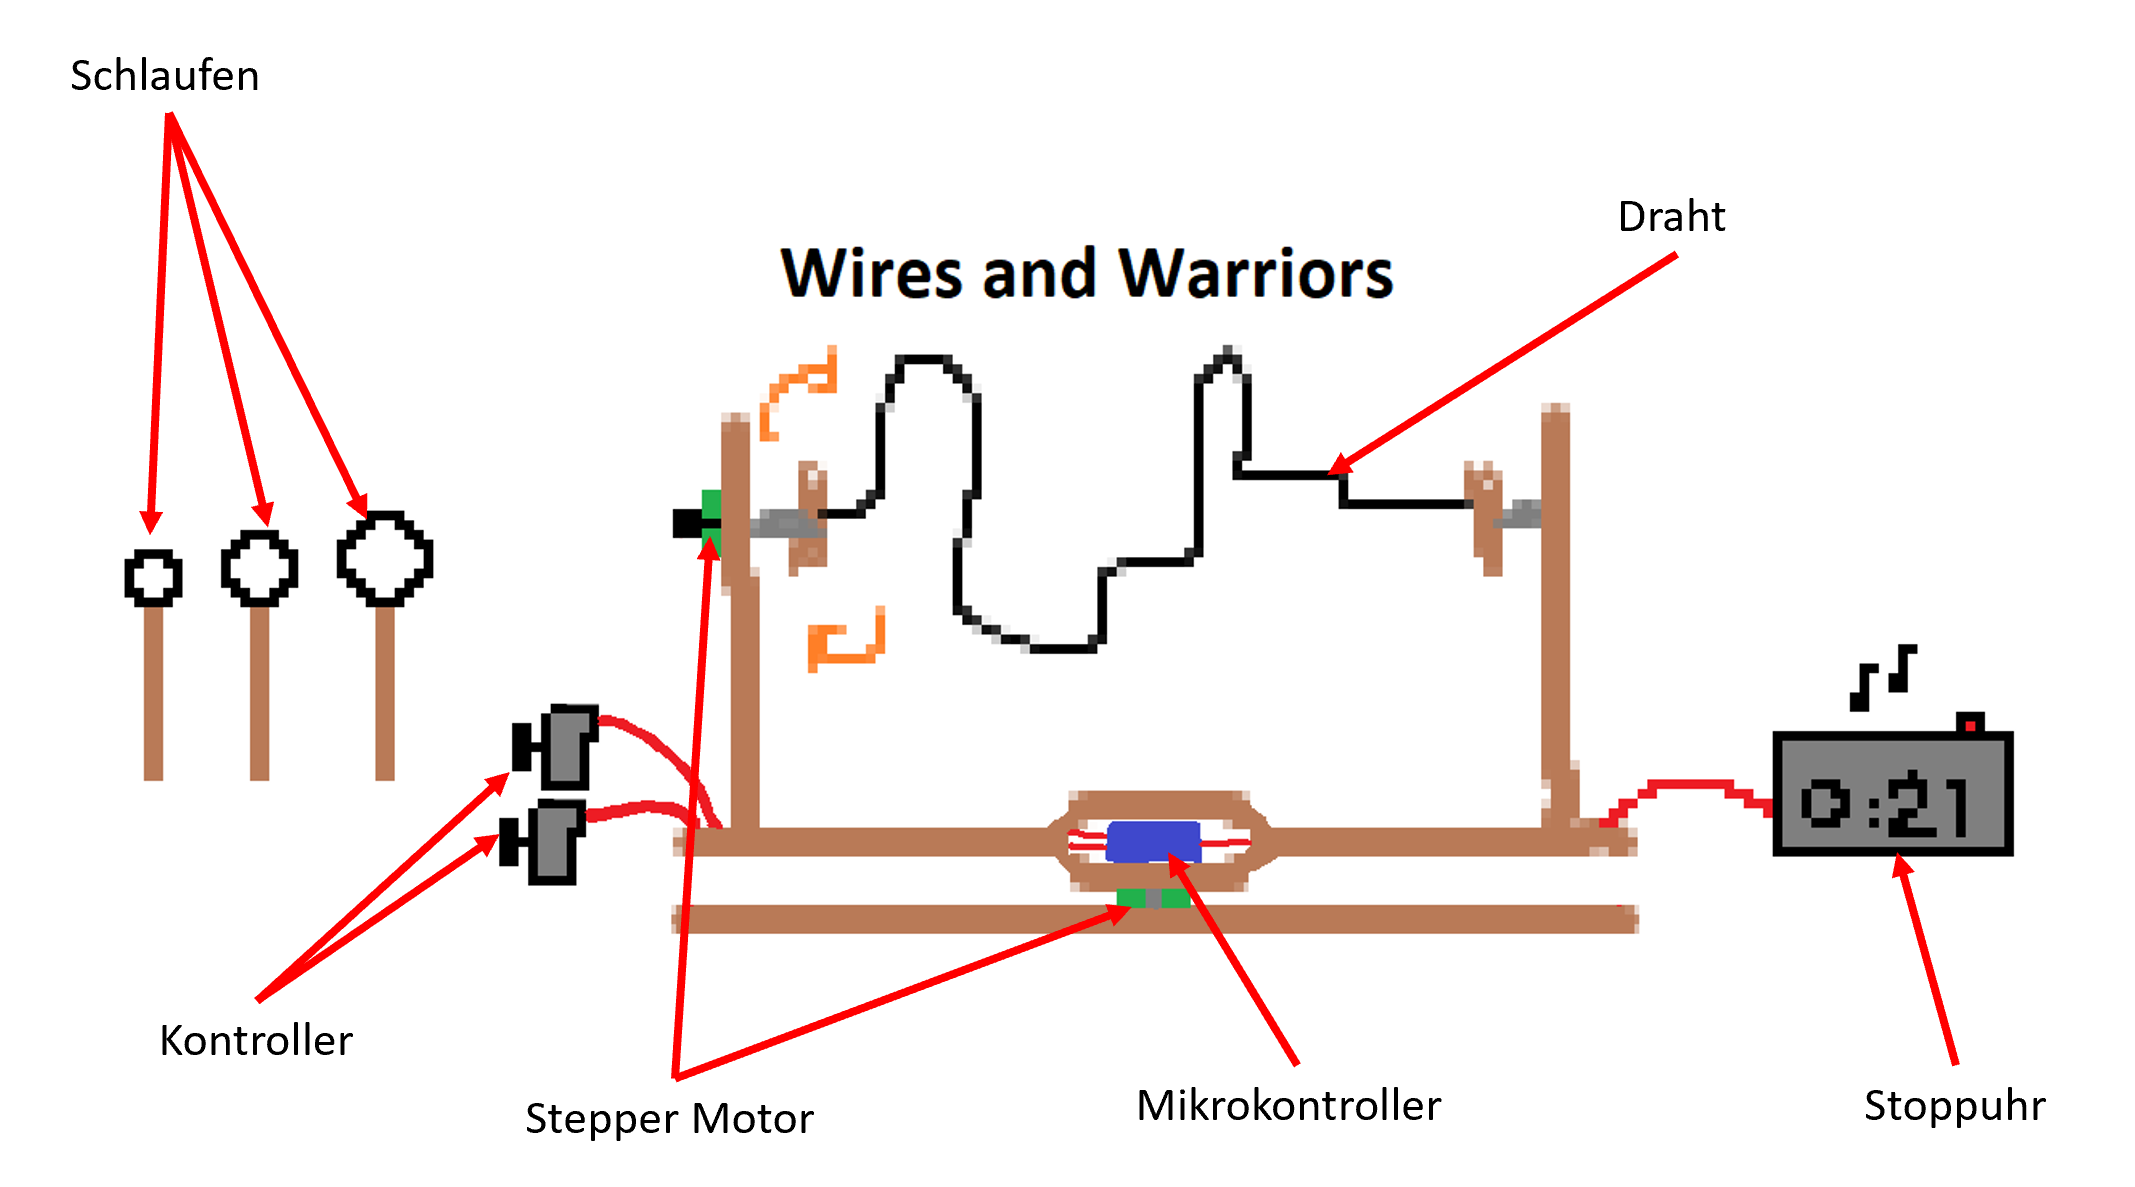
\includegraphics[width=0.75\textwidth,scale=1]{./images/Konzeptpapier_1.png}}
 \caption{Visualisierung des ersten Konzepts}\label{imageLabel}
\end{figure}  

\textbf{Zweite Konzept}: Dieses System sollte drei separate Drähte nutzen: einer rechts, einer links und einer in der Mitte als Brücke. Die äußeren Drähte sollten sich um die Y-Achse und das Mittelstück um die X-Achse drehen können. Das Ziel ist es gewesen, die gegenüberliegende Seite zu erreichen. Die Herausforderung bestand darin, dass die Spieler sich koordinieren mussten, um das Spiel zu beenden. Dieses Konzept war nicht ausgereift, jedoch bietet sie ein vielversprechendes Grundkonzept für die weitere Entwicklung. Der Entwurf des Systems sah wie folgt aus:

\begin{figure}[H]
 \centerline{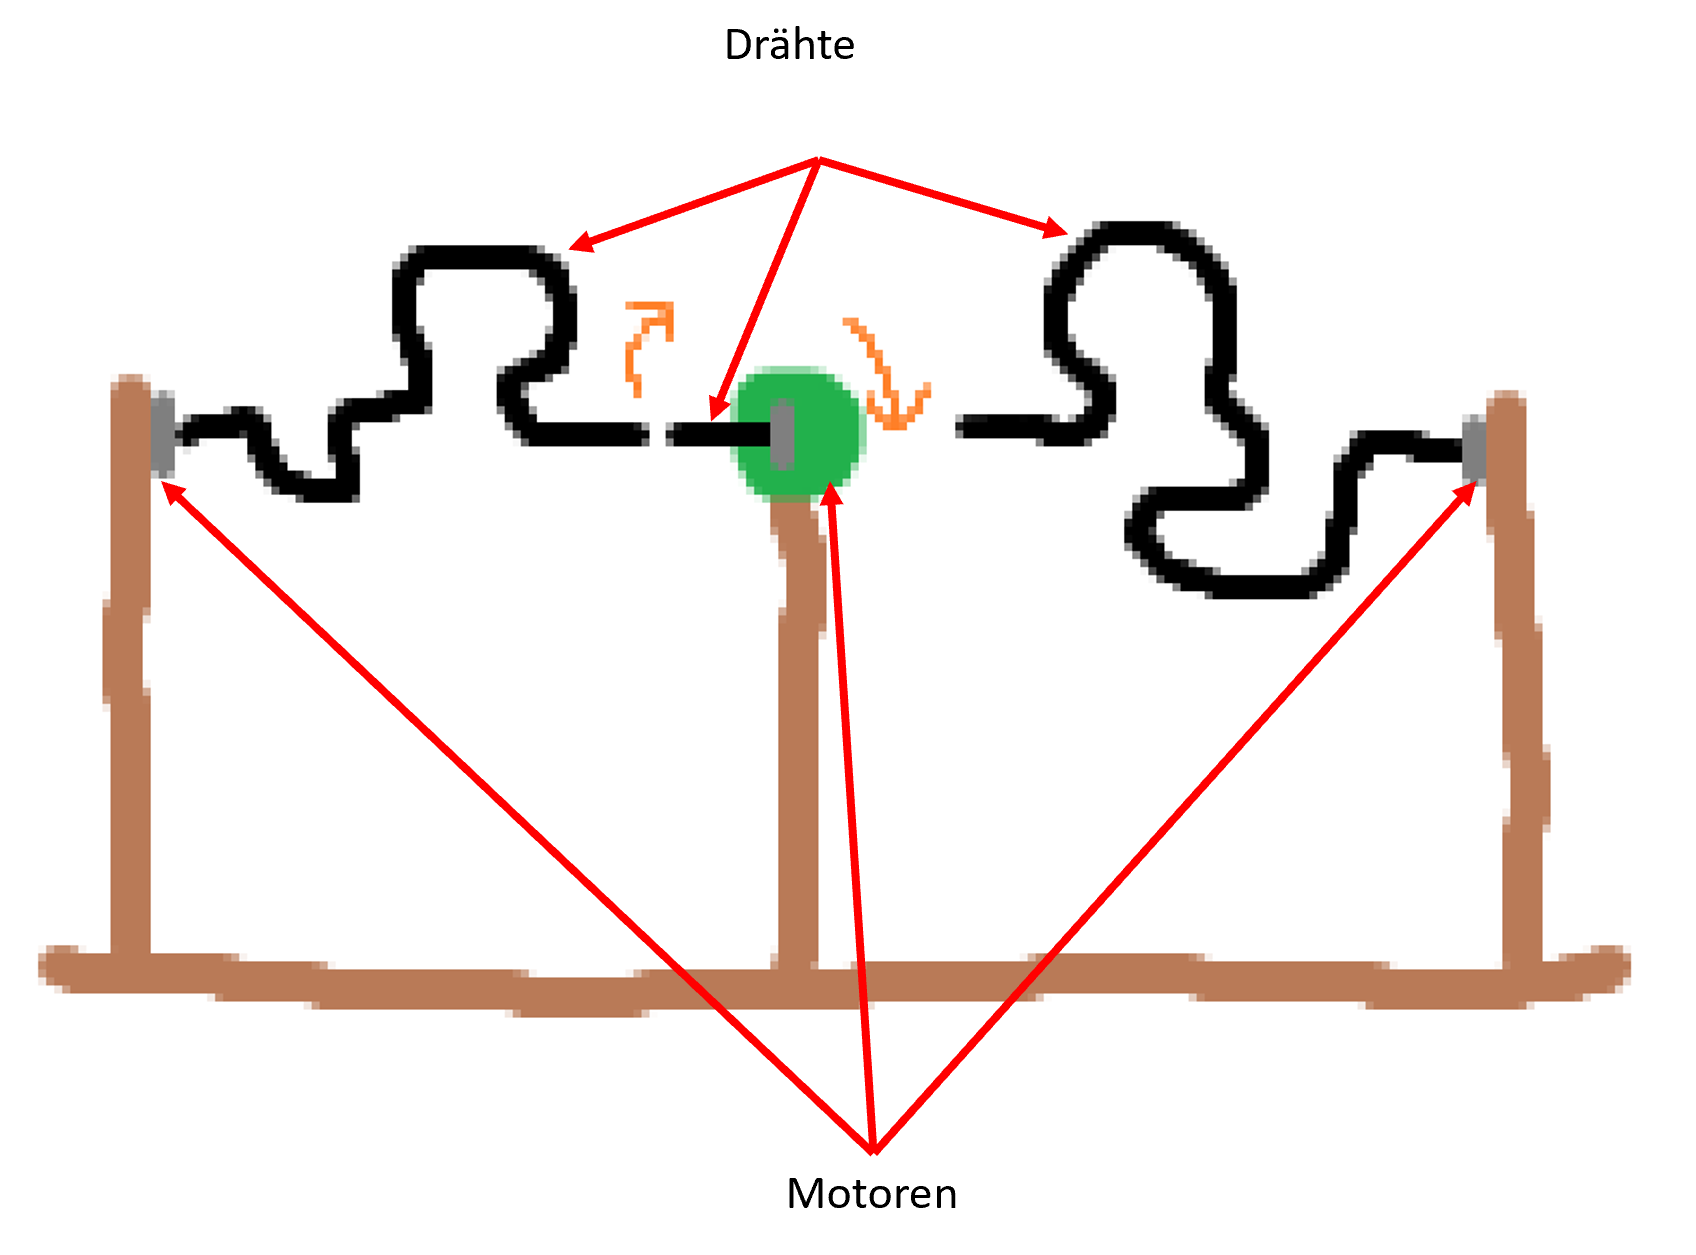
\includegraphics[width=\textwidth,scale=1]{./images/Konzeptpapier_2.png}}
 \caption{Visualisierung des zweiten Konzepts}\label{imageLabel}
\end{figure} 


\textbf{Dritte Konzept}: Das dritte Konzept sollte zwei Drähte besitzen. Diese wurden von den Seiten bis zur Mitte gespannt und am Mittelturm befestigt werden. Beide Spieler mussten, jeweils von den äußeren Seiten in die Mitte gelangen. Es zusätzlich möglich gewesen das ein dritter Spieler das System kontrollieren konnte über Kontroller. Diese Kontroller haben es ihm ermöglicht, die zwei Drähte rotieren zu lassen. Dieses Konzept entsprach nicht dem Charakter eines Escape-Rooms und wurde verworfen. Der Entwurf des Systems sah wie folgt aus: 

\begin{figure}[H]
 \centerline{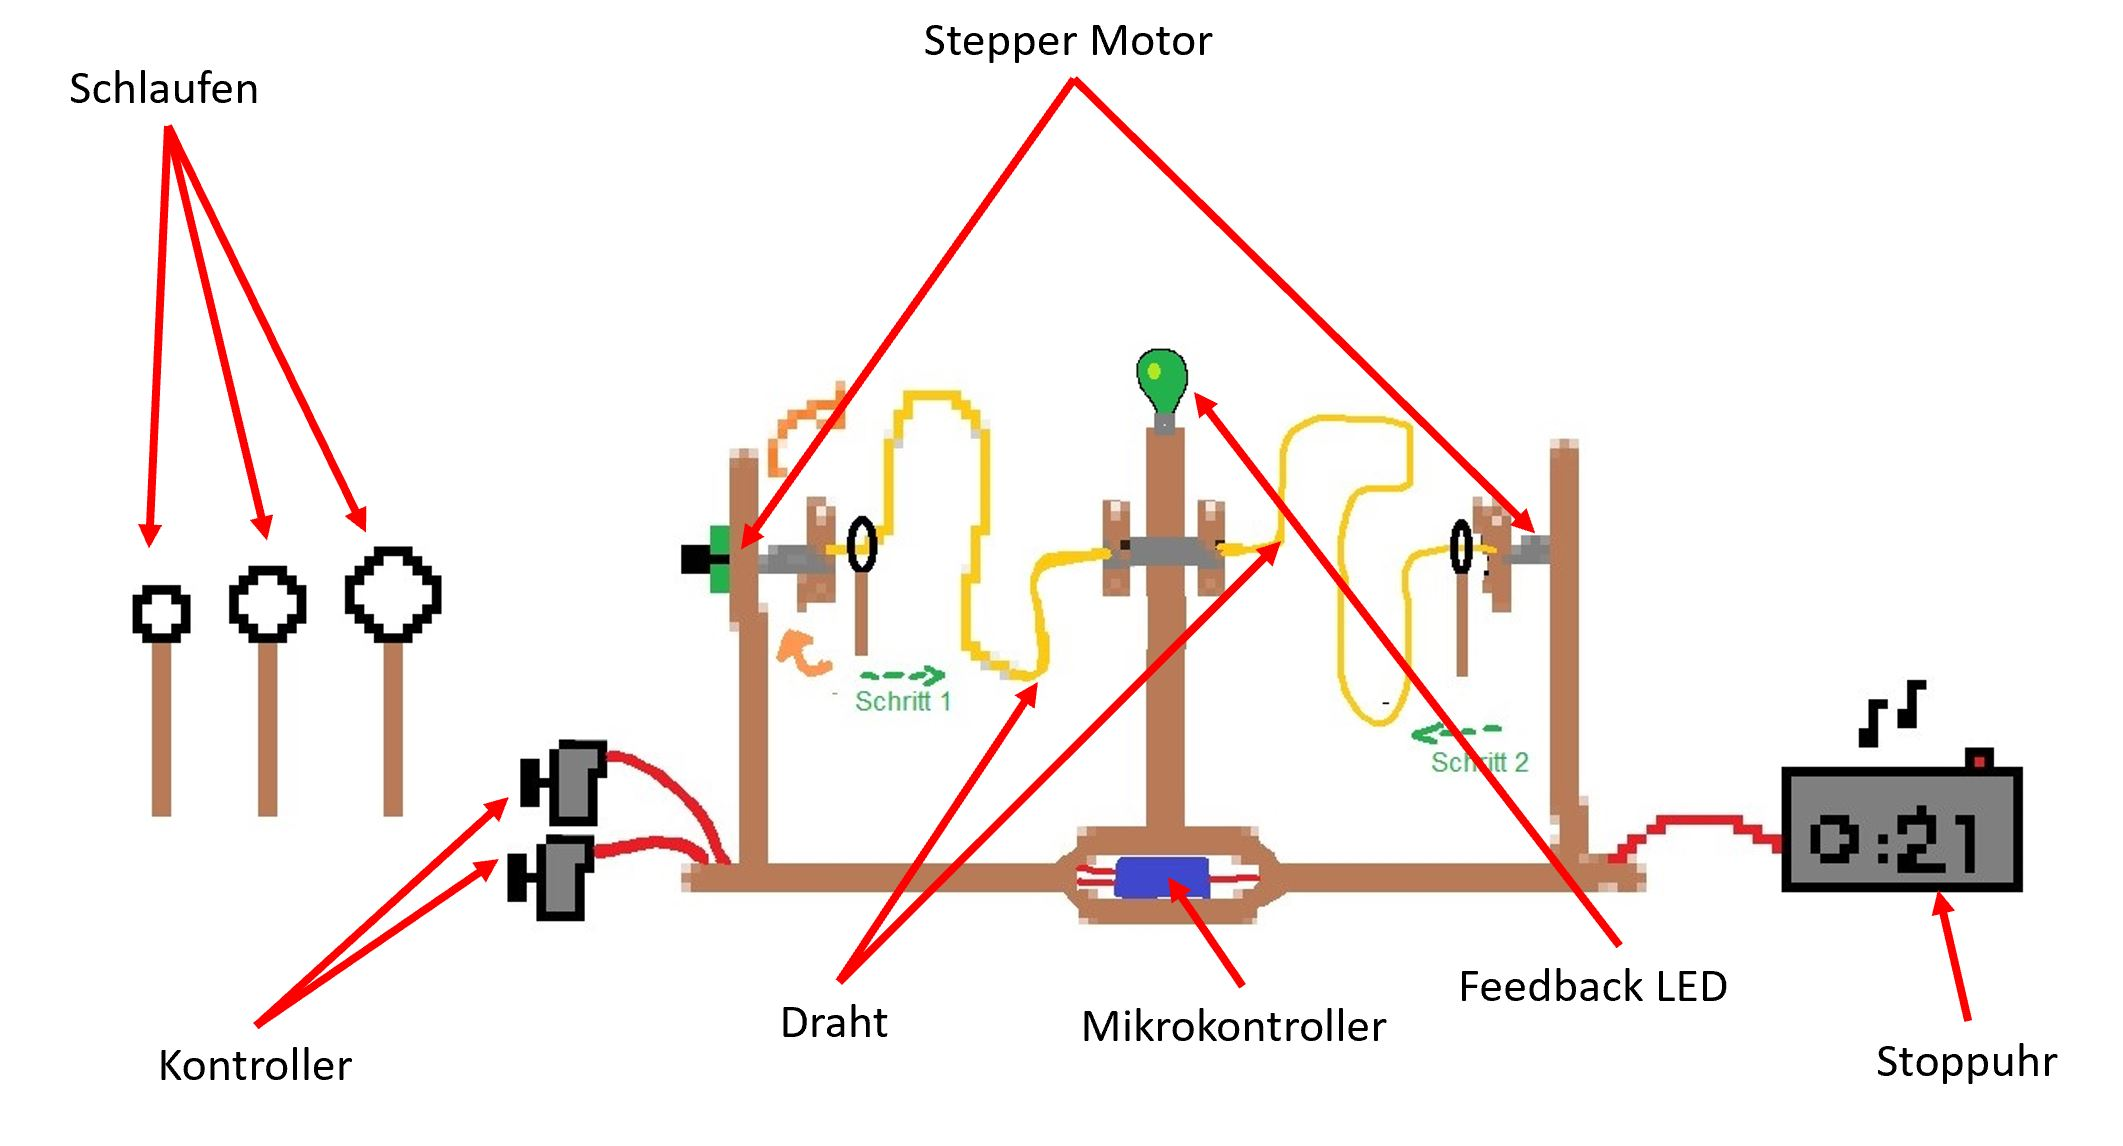
\includegraphics[width=\textwidth,scale=1]{./images/Konzeptpapier_3.jpg}}
 \caption{Visualisierung des dritten Konzepts}\label{imageLabel}
\end{figure} 


\textbf{Vierte Konzept}: Dieses Mal wurden die Türme auf einer Seite und die Brücke gegenüber platziert. Die Drahttürme rotieren um die Y-Achse und die Brücke um die X-Achse. Diese Idee wurde aufgrund mangelnder Nutzerfreundlichkeit schnell verworfen, jedoch wurde das Konzept des äußeren Gerüsts für das finale Design als Basis genutzt. Der Entwurf des Systems sah wie folgt aus:

\begin{figure}[H]
 \centerline{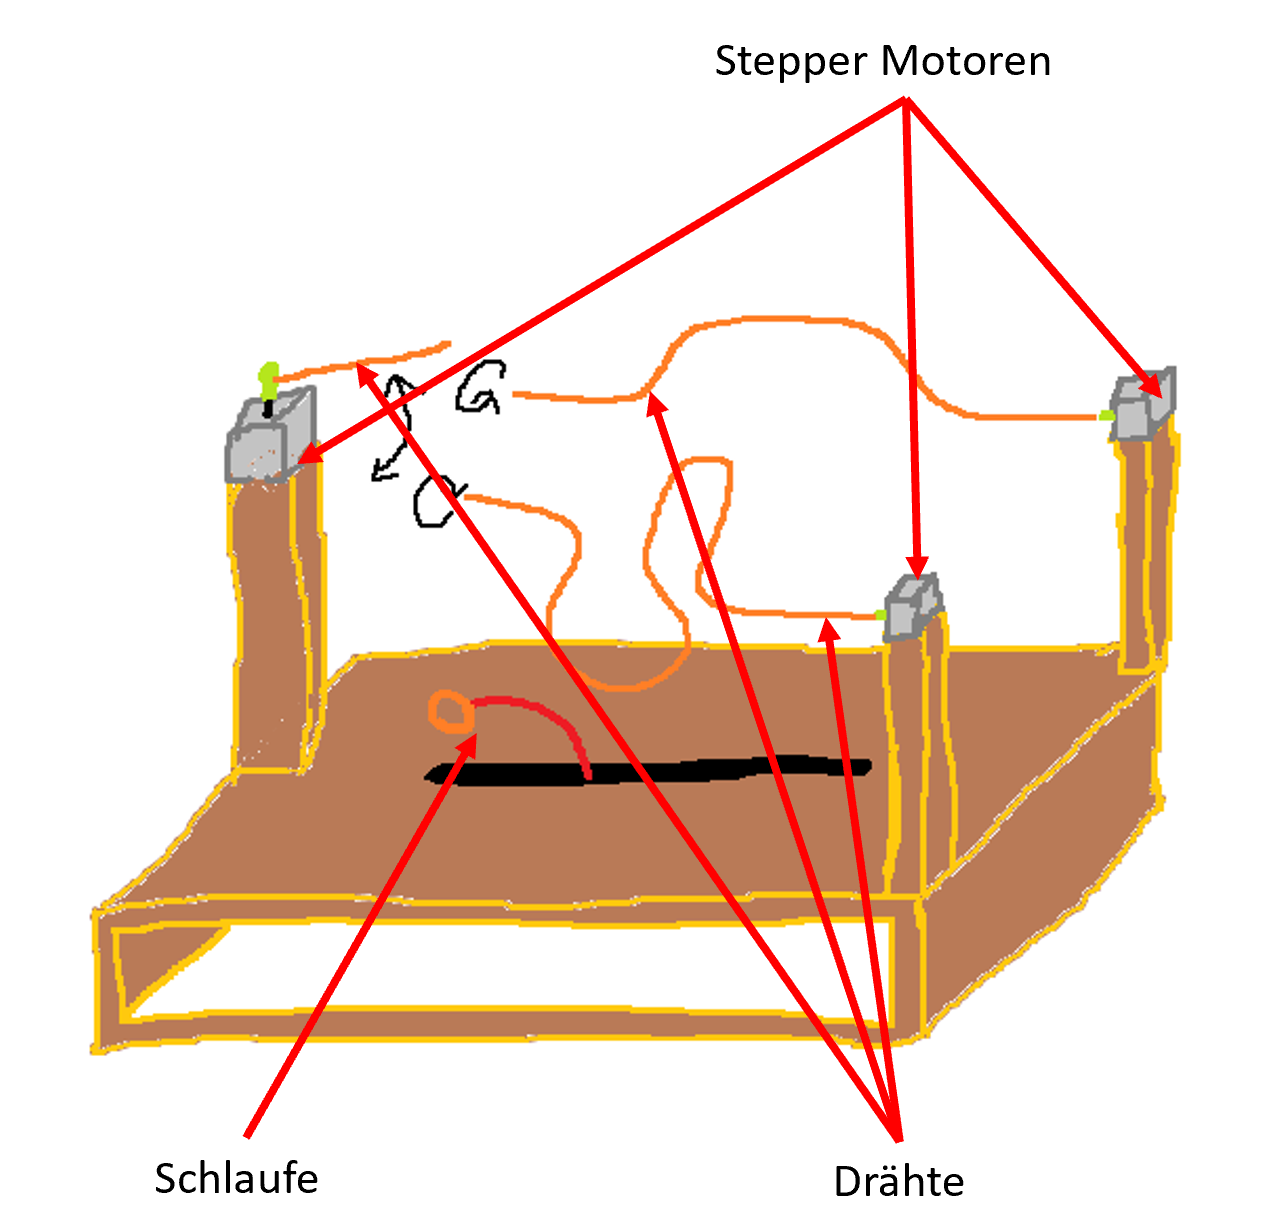
\includegraphics[width=.6\textwidth,scale=1]{./images/Konzeptpapier_6.png}}
 \caption{Visualisierung des vierten Konzepts}\label{imageLabel}
\end{figure} 

\textbf{Fünfte Konzept}: Das letzte Konzept ist eine Kombination aus dem dritten und zweiten Ansatz gewesen. Es gibt zwei Spieler, die gegen das System antreten, mit drei Drähten: links, rechts und ein Mittelstück. Die äußeren Drähte drehen sich um die Y-Achse, das Mittelstück um die X-Achse. Das System sollte ein Startknopf, Fehler-LEDs und Herzen zur Spieler-Rückmeldung besitzen. Die Spieler starten an den äußeren Türmen und müssen auf die andere Seite gelangen. Dieses Konzept war erfolgversprechend und wurde als Grundkonzept genommen und ausgearbeitet. Der Entwurf des Systems sah wie folgt aus:

\begin{figure}[H]
 \centerline{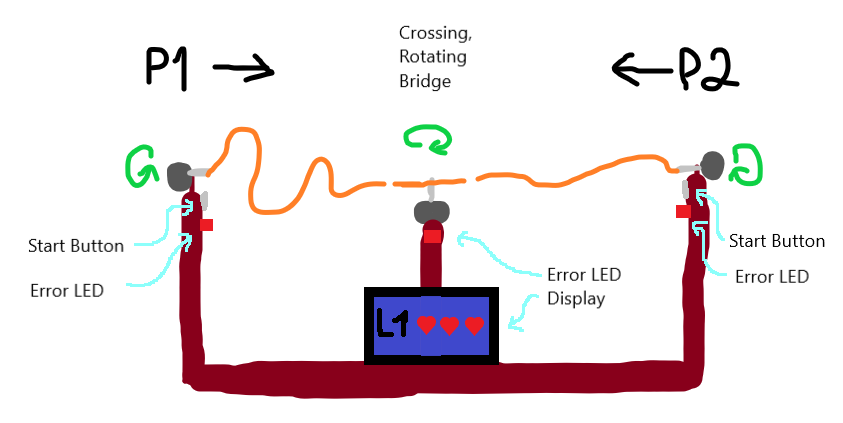
\includegraphics[width=\textwidth,scale=1]{./images/Konzeptpapier_5.png}}
 \caption{Visualisierung des fünfte Konzepts}\label{imageLabel}
\end{figure} 

\section{Modellierung des 3D-Design}

Bei der Modellierung des 3D-Designs für Wire \& Warriors wurde auf ein modulares System geachtet. Die Modularität war ein zentraler Aspekt des Designs, denn dadurch war es möglich die Komponenten für Wartung und Upgrade leicht zugänglich zu machen.

Das gesamte Gerüst des Spieles musste aufgrund der Größenbeschränkung der Holzplatten, jeweils 30x60 Zentimeter groß, durchdacht werden. Die Verwendung von Verzahnung im Modell war ein wichtiger Bestandteil. Diese Bauweise ermöglicht es, dass einzelne Platten fest eineinander greifen konnten, wodurch eine stabile Struktur ohne zusätzliche Verbindungselemente wie Schrauben oder Nägel zu schaffen. Diese Verzahnung sahen wie folgt aus:


\begin{figure}[H]
 \centerline{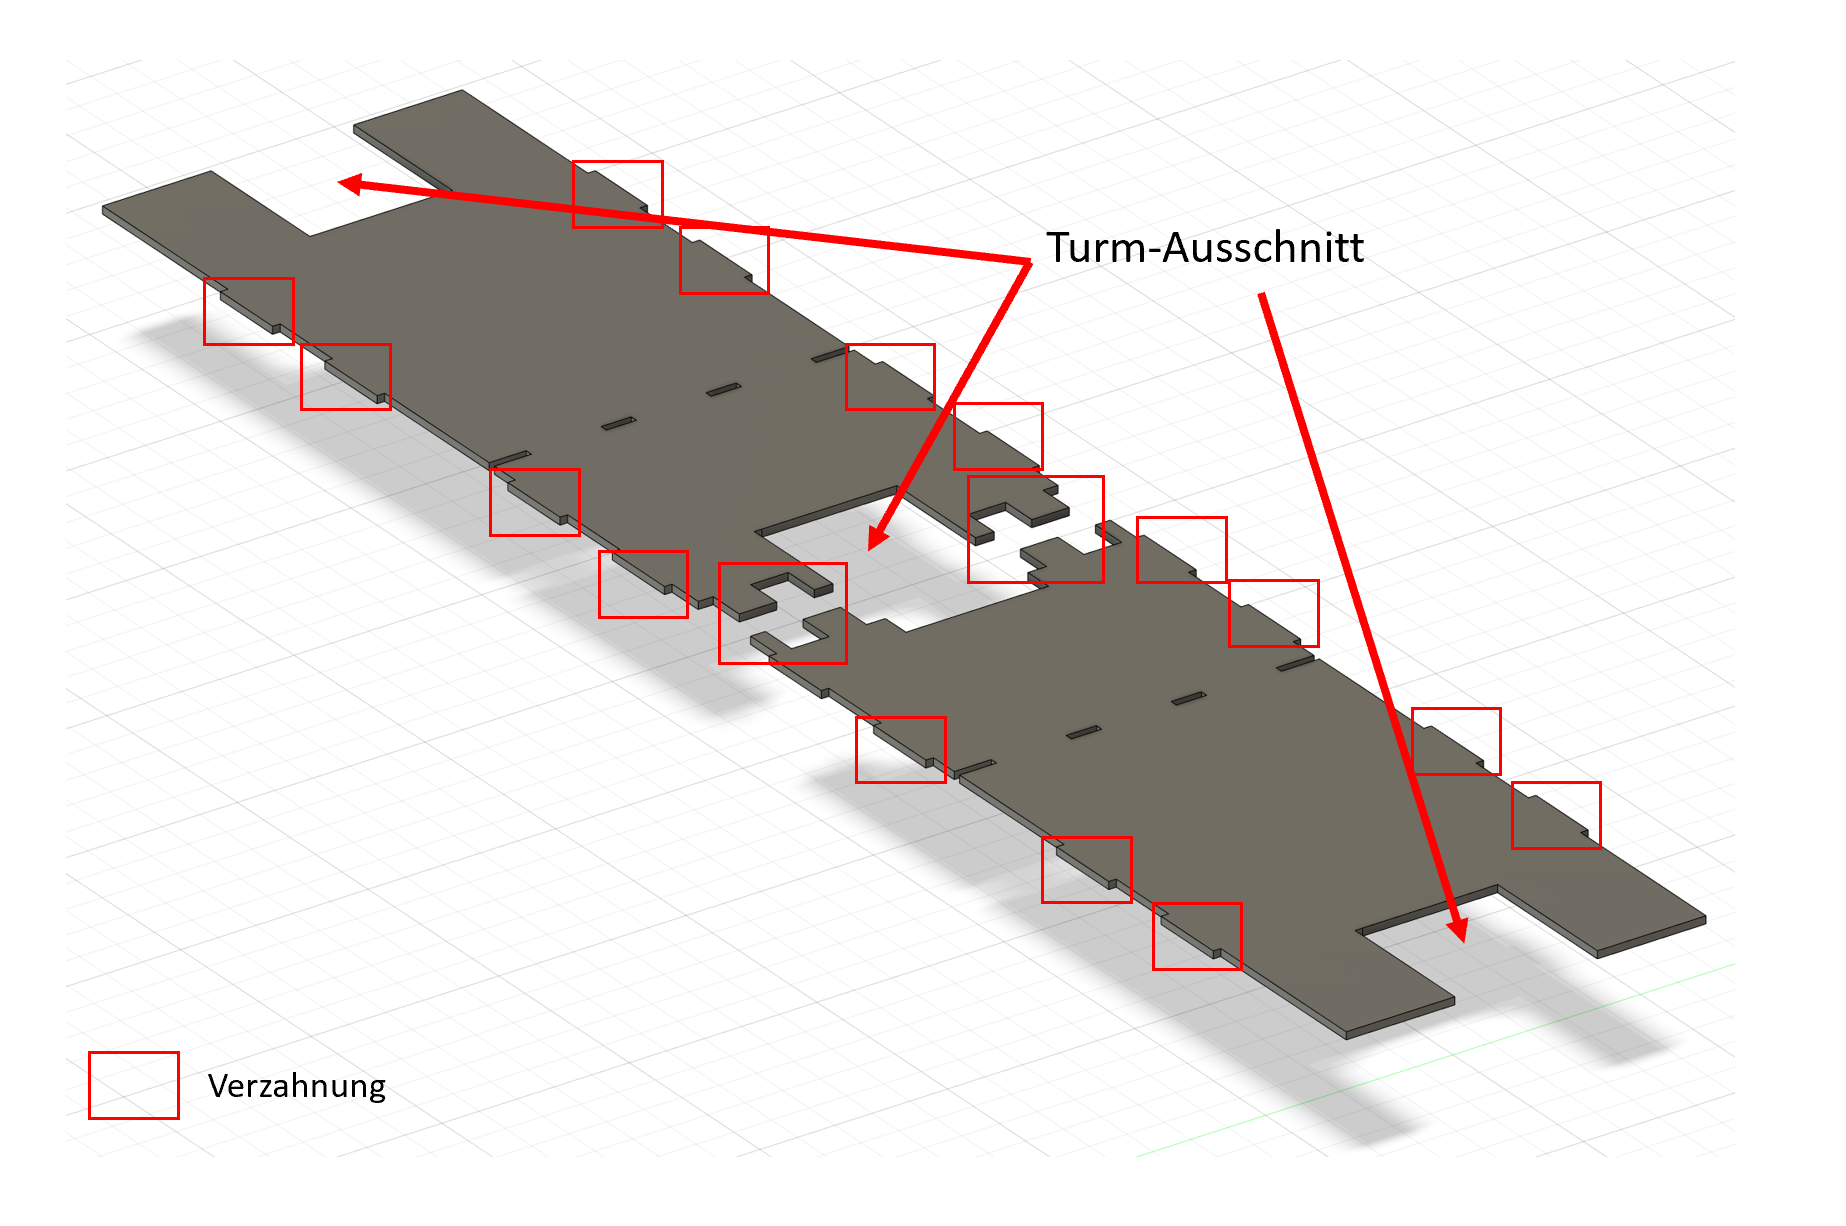
\includegraphics[width=\textwidth,scale=1]{./images/verzahnung.png}}
 \caption{Verzahnung am Deckel}\label{imageLabel}
\end{figure} 

Zusätzlich wurde des gesamt Gerüst durch die Mittelstücke, die auch als Kabelführung gedient haben, verstärkt. Die Mittelstücke wurden im Deckel, in den Wänden und am Boden angebracht. Diese Mittelstücke sehen wie folgt aus:

\begin{figure}[H]
 \centerline{\includegraphics[width=0.75\textwidth,scale=1]{./images/mittelstück.png}}
 \caption{Stabilisierung des Gerüstes durch Mittelstücke}\label{imageLabel}
\end{figure} 

Die Türme des Spieles wurden in das Gerüst eingesetzt und wurden durch die Deckel befestigt. Jeder Turm hatte einen Ausschnitt für den Stepper-Motor und eine Ablage. Die Türme sahen wie folgt aus:

\begin{figure}[H]
 \centerline{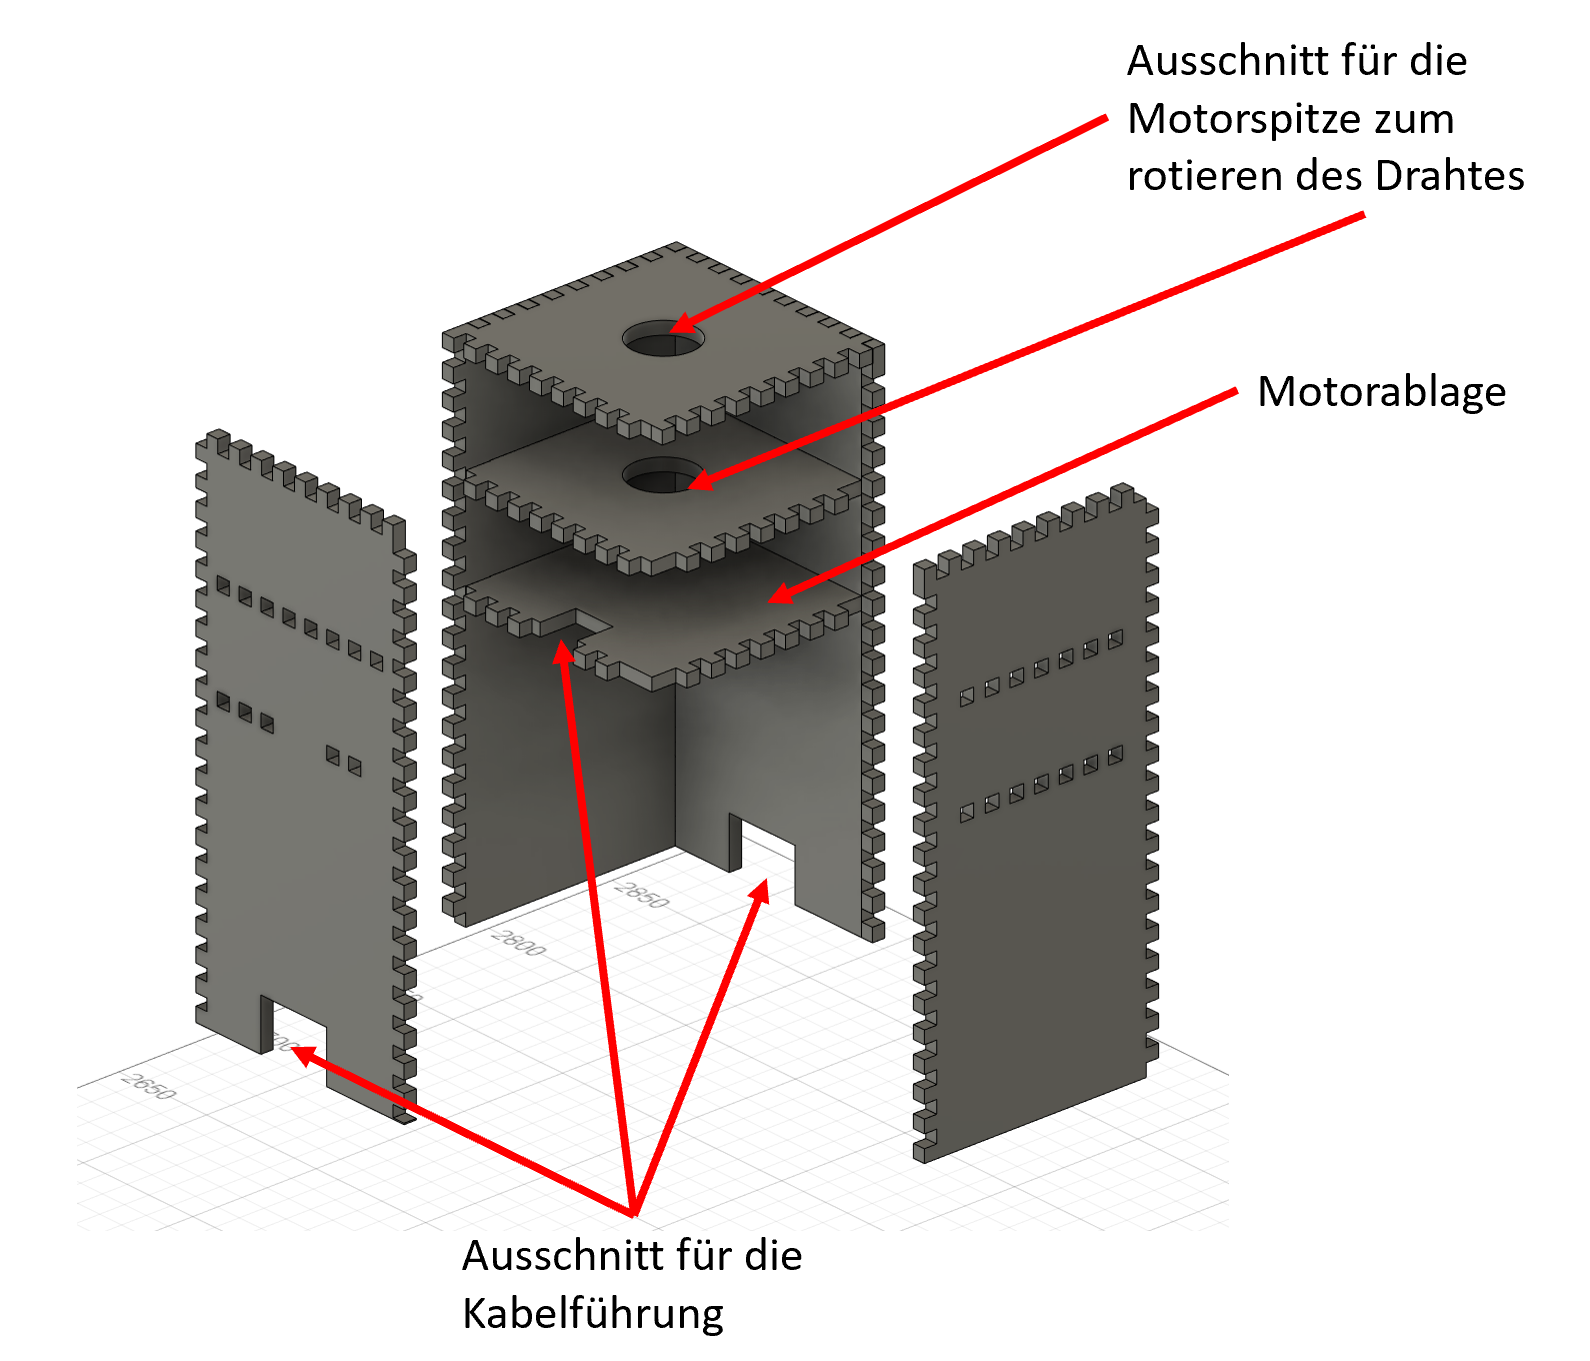
\includegraphics[width=0.75\textwidth,scale=1]{./images/turm_mitte.png}}
 \caption{Einblick in den mittleren Turm}\label{imageLabel}
\end{figure} 


Das gesamte Design diente als Vorlage für die Laserauschnitte, die später aus den Holzplatten gefertigt wurden. Diese Vorbereitung ist entscheidend gewesen, damit alle Teile Präzise zusammenpassen. 

Die Modularität und die leichte Zugänglichkeit der Komponenten sorgt für eine einfach Wartung bzw. Upgrades. Das hat den Vorteil, dass eine schnelle Anpassung z.B. an neue Spielvariaten möglich wäre. Das Endresultat ist ein durchdachtes und funktionales 3D-Design und sieht wie folgt aus: 

\begin{figure}[H]
 \centerline{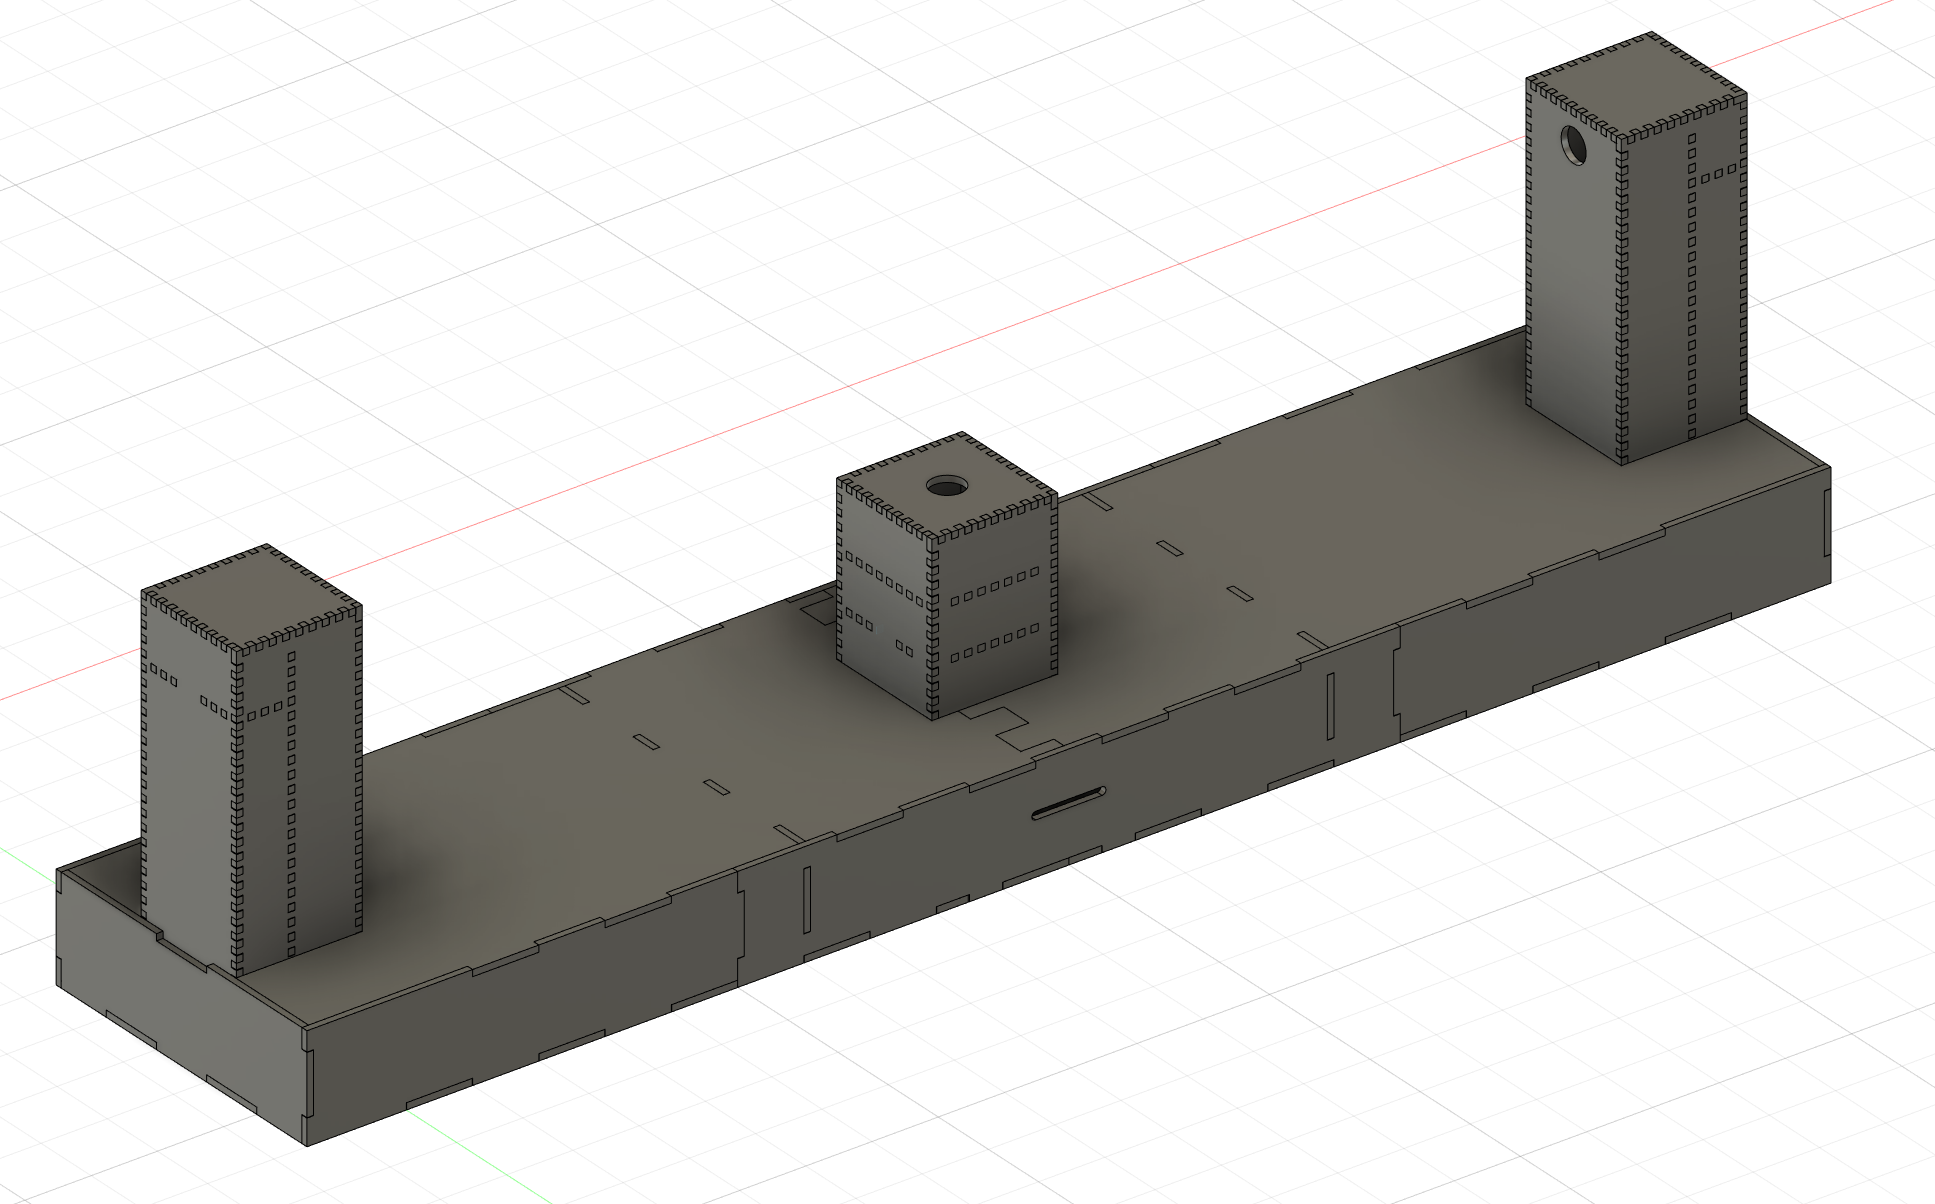
\includegraphics[width=\textwidth,scale=1]{./images/gesamt_design.png}}
 \caption{Das gesamte Design für Wire \& Warriors}\label{imageLabel}
\end{figure} 


  \chapter{Hardware Umsetzung}

Für die Umsetzung von Wire \& Warriors wurden verschiedene Hardwarekomponenten ausgewählt und integriert. Es sind folgende Komponenten genutzt für die Realisierung:

\textbf{Stepper-Motorn}: Diese Komponenten wurden für die präzisen Bewegungen der Drähte genutzt. Es sind drei Motorn\cite{Tronxy3DPrinter2023} zum Einsatz gekommen: linker Turm, rechter Turm und mittlerer Turm. Dadurch ist es möglich gewesen, die Drähte rotieren zu lassen und die Geschwindigkeit anzupassen.

\textbf{Messingdrähte}: Die Drähte\cite{hagebauGAHALBERTSRundstange2023} sind ein Meter lang gewesen und hatten einen Durchmesser von 6 Millimetern. Die Messingdrähte wurden gewählt, da sie eine gute Balance zwischen Flexibilität und Festigkeit bieten. Zusätzlich besitzt Messing eine gute elektrische Leitfähigkeit, dass ist wichtig gewesen um Berührungen von Spielern zu detektieren.

\textbf{Stepper-Treiber TB6600}: Um die Motorn zu steuern, wurden drei TB6600 Stepper-Treiber\cite{dfrobotTB6600_Stepper_Motor_Driver_SKU__DRI0043DFRobot2023} eingesetzt. Die Treiber ermöglichen die präzise Steuerung der Motorn. Dadurch ist es möglich gewesen, die Motorn gleichmäßig und kontrolliert zu bewegen. Ein enormer Vorteil dieser Treiber ist gewesen, dass sie einfach konfigurierbar durch seitliche Schalter sind. Somit ist es möglich gewesen, die Treiber einfach und schnell auf die Motorn einzustellen.

\textbf{Soundmodul}: Ein Soundmodul ist hinzugefügt worden, um akustisch Feedback für die Spieler zu geben. Dies sollte zur Spielatmospähre beitragen und die Benutzerfreundlichkeit erhöhen.

\textbf{Netzteil}: Es wurde ein Netzteil verbaut, um die Mobilität des Spiels zu gewährleisten. Dadurch kann das Spiel jederzeit flexible an verschiedenen Orten genutzt werden.

\textbf{LEDs}: Es wurden acht LEDs integriert, um visuelles Feedback zu geben. Damit konnten wichtige Spielinformationen wie Spielstatus und die verbleibende Herzen den Spielern angezeigt werden.


\textbf{Arduino Uno-Einsatz}: Dieser Mikrocontroller diente als zentrale Steuereinheit des Spiels. Der Adruino Uno ermöglicht die Steuerung der Stepper-Motoren, das Detektieren von Berührungen und die Ansteuerung der visuellen und akustischen Rückmeldungen durch LEDs und das Soundmodul.

\section{Prototypen}

Mit diesen Komponenten ist es möglich gewesen, das Spiel Wire \& Warrios zu realisieren. Für die ersten Annäherung zur Realisierung des Spieles wurde Prototypen entwickelt. Der erste Prototype sah wie folgt aus:

\begin{figure}[H]
 \centerline{\includegraphics[width=\textwidth,scale=1]{./images/prototype_1.png}}
 \caption{Die Umsetzung des Prototypens zum detektieren von Berürhungen}\label{prototype_1}
\end{figure}

Der erste und simpelste Prototype, wie in der Abbildung \ref{prototype_1} zu sehen, ermöglichte die Detektierung von Berührungen. Die Berührungen wurden durch die rote LED signalisiert. Der nächste Schritt ist gewesen einen Motor einzubauen, um den Draht zu bewegen. Dieser Prototyp sah wie folg aus:


\begin{figure}[H]
 \centerline{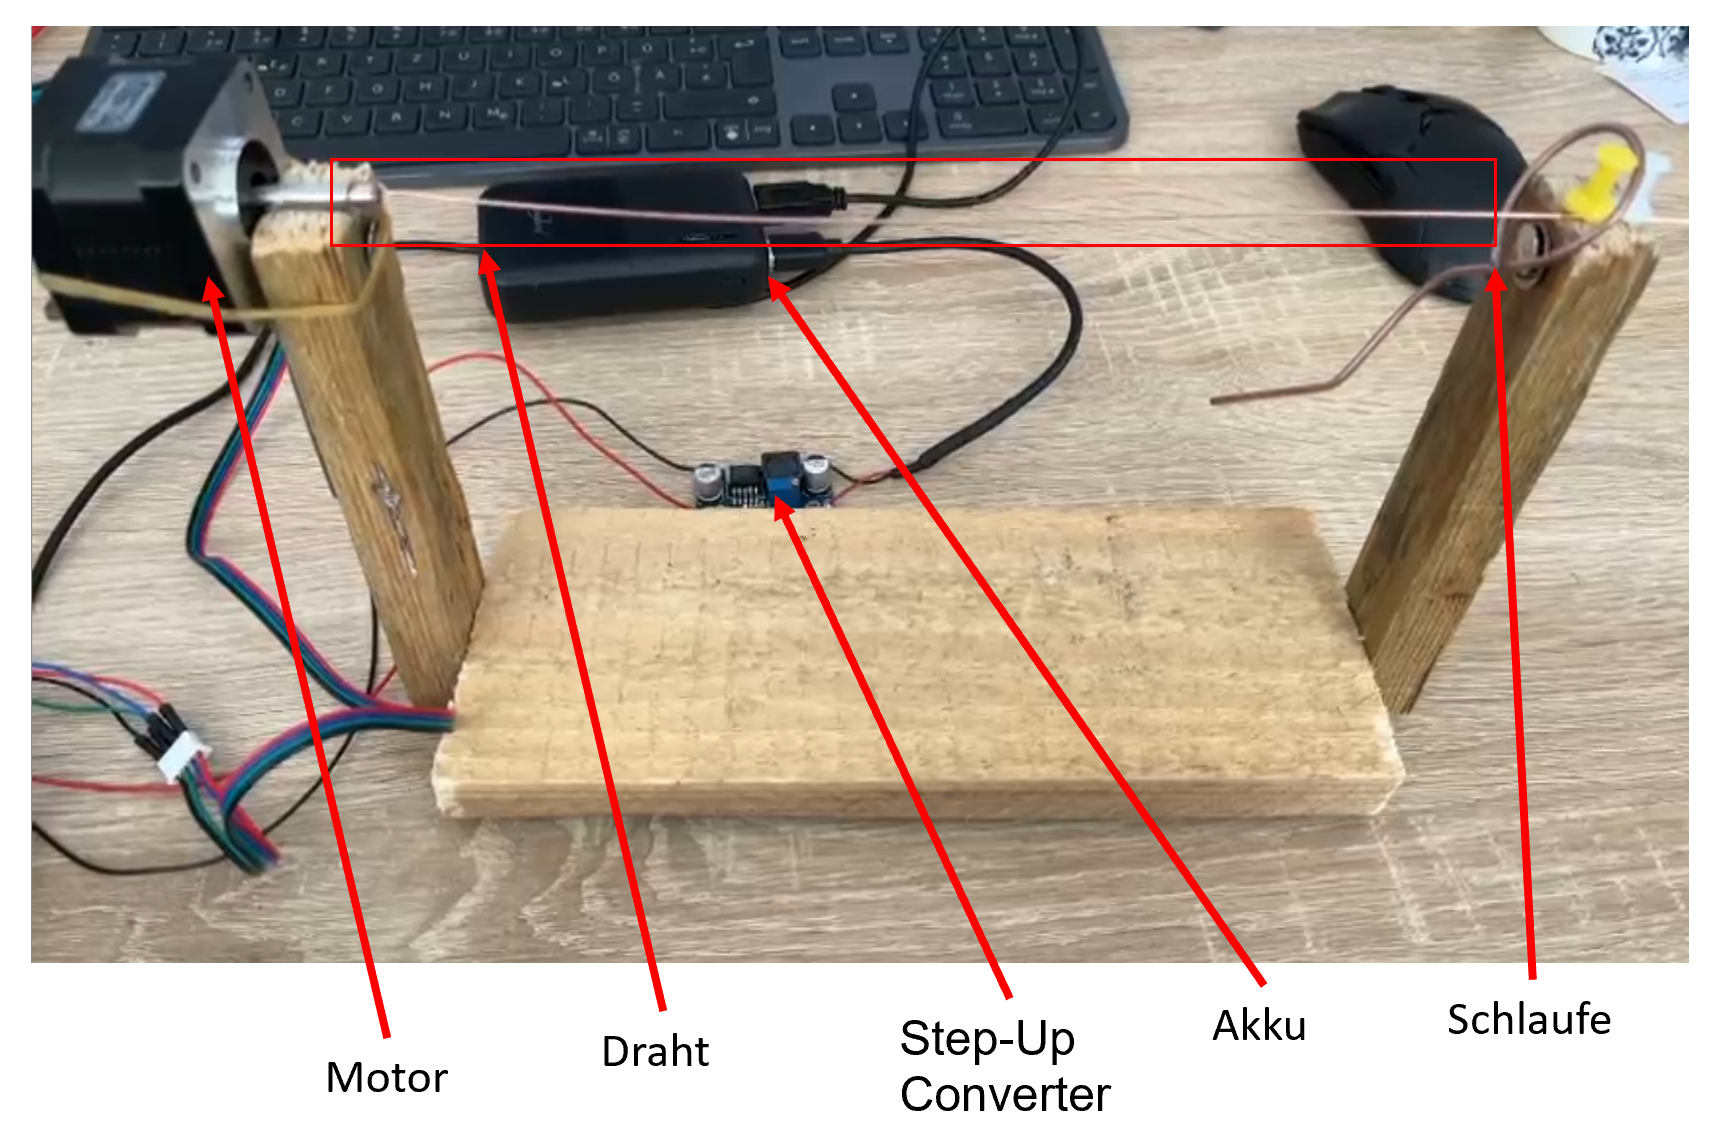
\includegraphics[width=\textwidth,scale=1]{./images/prototype_2.png}}
 \caption{Die Umsetzung des Prototypens}\label{prototype}
\end{figure} 

Mit dem zweite Prototype, in der Abbildung \ref{prototype} zu sehen, ist es möglich gewesen, den Draht zu drehen und Berührungen zu detektieren. Der Step-Up Converter wurde genutzt, um die notwendige Spannung für den Stepper-Motor zu erreichen. Dieser konnte nicht allein durch die Ausgangsspannung vom Akku erreicht werden. Der Step-Up Converter wurde im Endprodukt durch das Netzteil ersetzt.

Zusätzlich musste der Stepper Motor Driver integriert werden, um den Motor zu steuern. Das Schaltbild für die Integrierung sah wie folgt aus:

\begin{figure}[H]
 \centerline{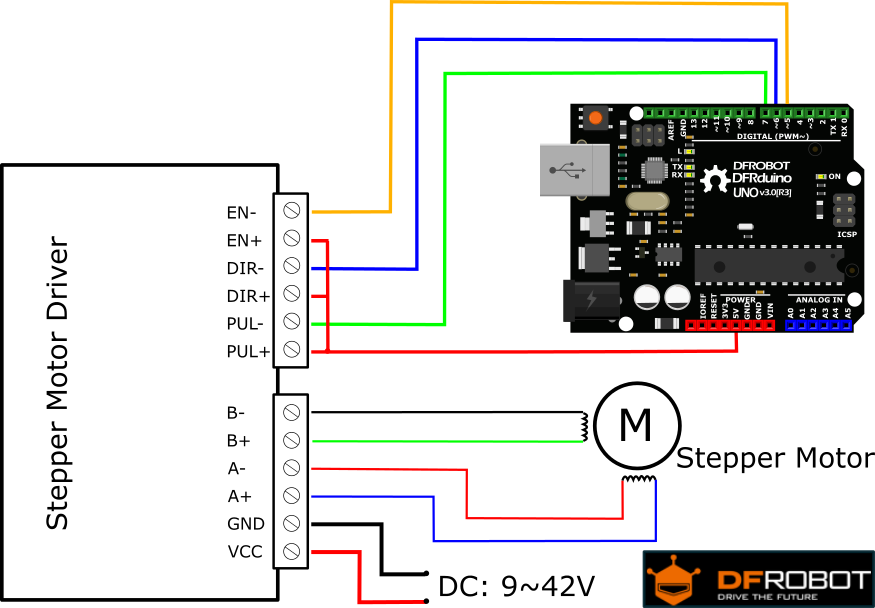
\includegraphics[width=\textwidth,scale=1]{./images/circuit_plan_stepper_motor_driver.png}}
 \caption{Schaltplan des Stepper Motor Drivers}\label{schaltplan_stepper}
 \caption*{Quelle: \href{https://wiki.dfrobot.com/TB6600_Stepper_Motor_Driver_SKU__DRI0043}{TB6600 Stepper Motor Driver}}
\end{figure} 

Der Schaltplan, wie in der Abbildung \ref{schaltplan_stepper} zu sehen, gibt die Verkabelung des Steppers vor. Bevor der Stepper Motor Driver genutzt werden konnte, musste die Stromstärke Konfiguration angepasst werden. Die Stepper Motorn haben eine Stromstärke von 1A benötigt und deshalb mussten die Schalter vier und sechs umgelegt werden. Die Konfigurationen stehen auf dem Stepper Motor Driver und sahen wie folgt aus:

\begin{figure}[H]
 \centerline{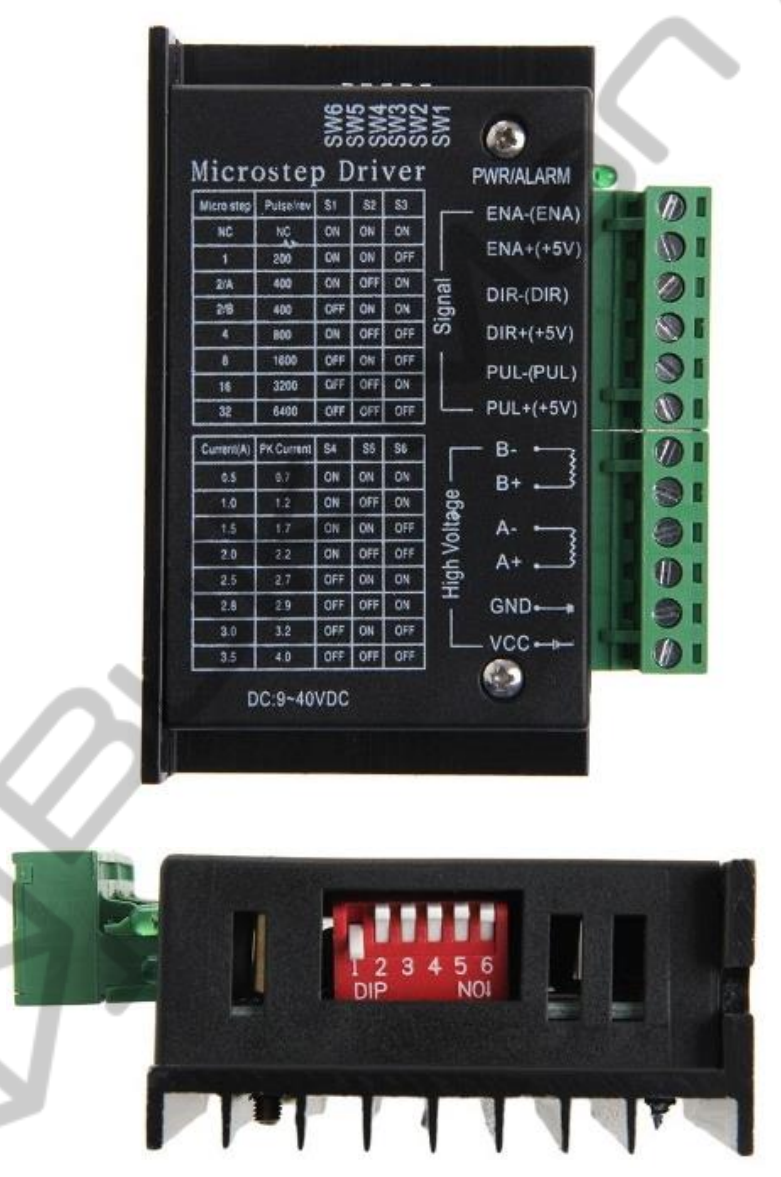
\includegraphics[width=0.45\textwidth,scale=1]{./images/stepper_motor_driver.png}}
 \caption{Konfigurationen auf dem Driver}\label{stepper}
 \caption*{Quelle: \href{https://bulkman3d.com/wp-content/uploads/2019/06/TB6600-Stepper-Motor-Driver-BM3D-v1.1.pdf}{TB6600 Stepper Motor Driver}}
\end{figure} 


Die Ausgänge vom Stepper Driver Motor `EN' und `DIR' wurden nicht genutzt, da die Drähte sich nur eine Richtung drehen sollen. Die Drehung wurde durch Ausgang `PUL' ermöglicht. Die Kabel aus `PUL' wurden am Arduino Uno angebracht.

\section{Realisierung des Projekts}

Das gesamte Gerüst hat eine Länge von einem Meter und eine Breite von 30 Zentimeter. Diese Größe ist kompakt und  bietet eine ausreichend große Spielfläche. Das zusammengebaute Gerüst sieht wie folgt aus:

\begin{figure}[H]
 \centerline{\includegraphics[width=0.25\textwidth,scale=1]{./images/gerüst.jpg}}
 \caption{Gerüst ohne Deckel}\label{turm}
\end{figure} 


Nachdem das Gerüst stand wurden die Türm fertiggestellt und sahen wie folgt aus:

\begin{figure}[H]
 \centerline{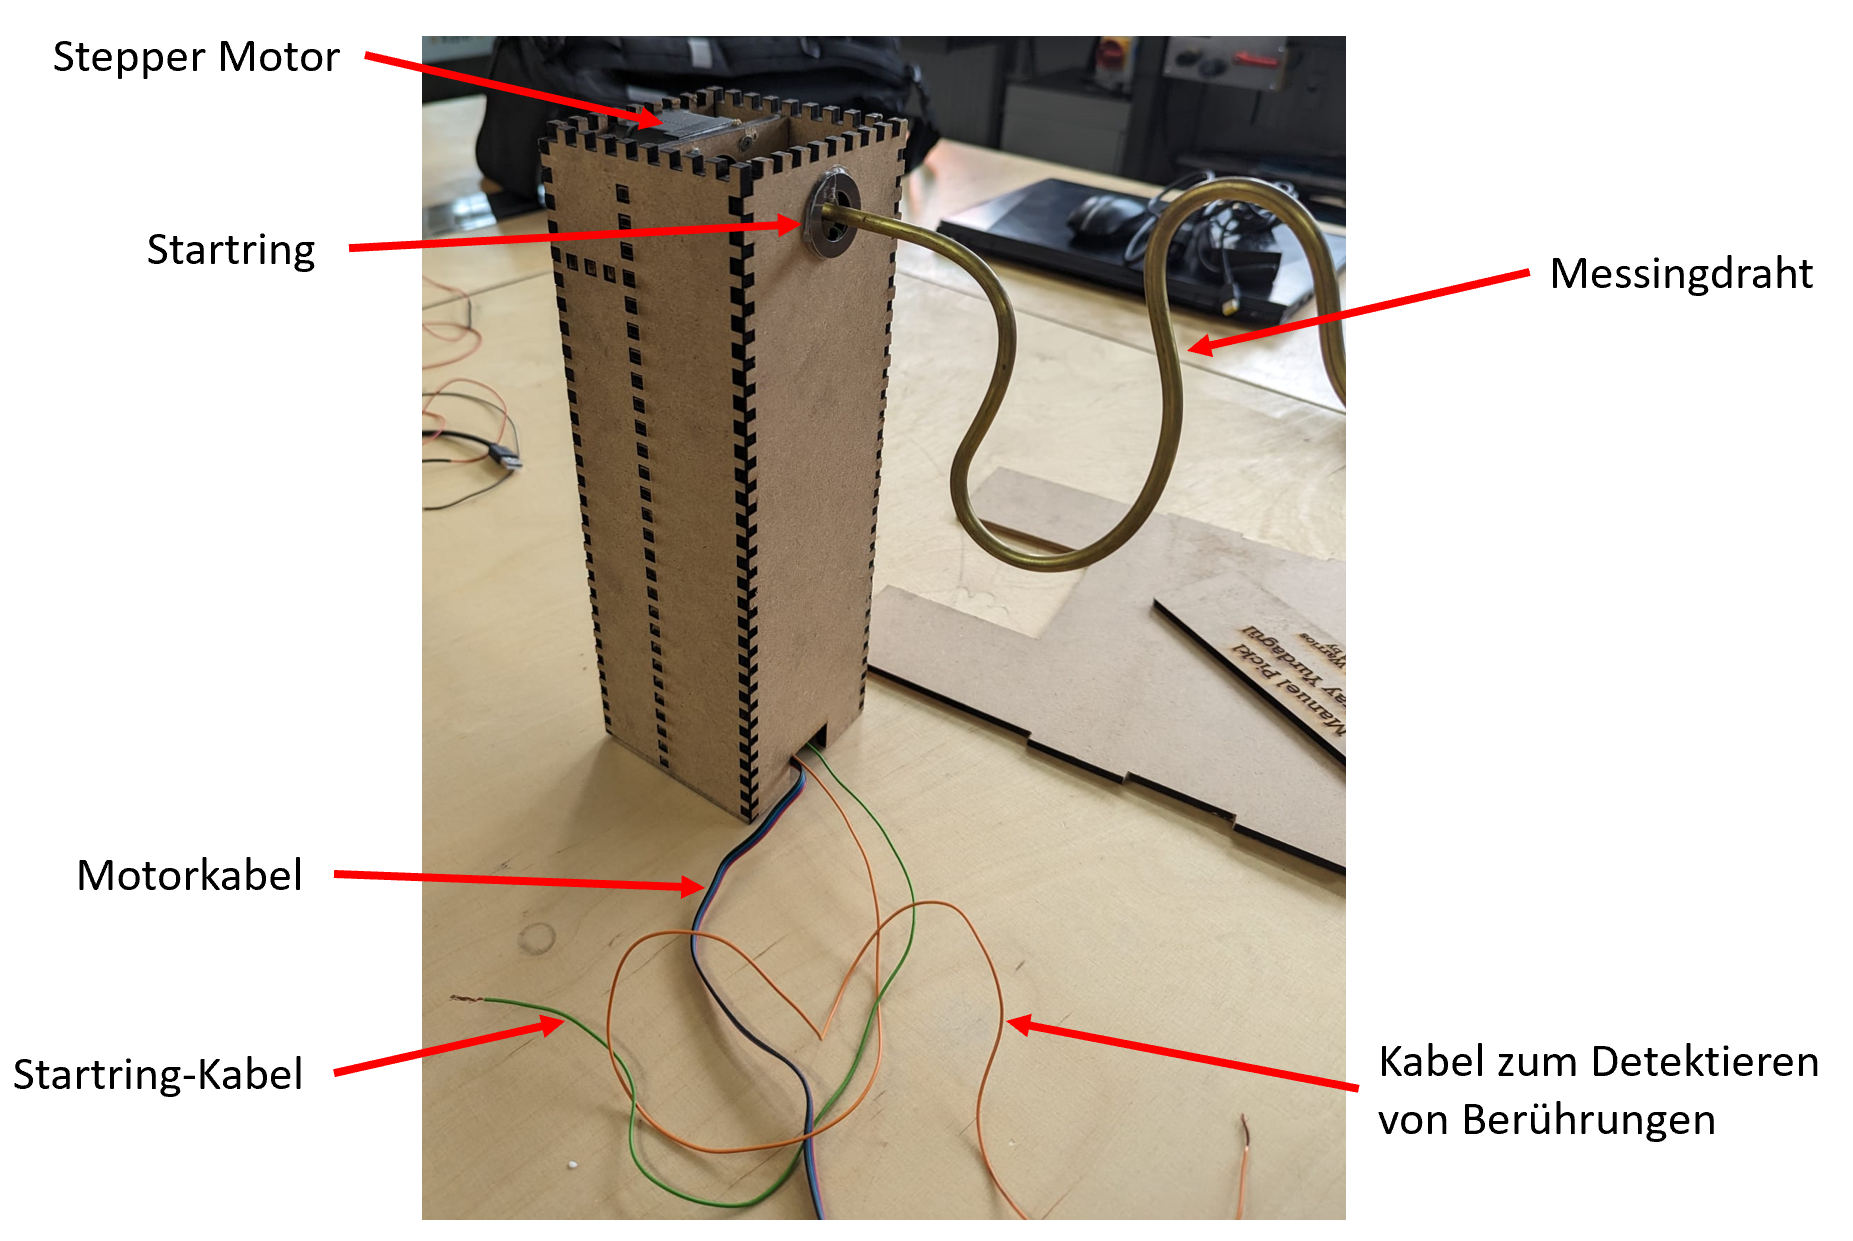
\includegraphics[width=.85\textwidth,scale=1]{./images/turm_holz.png}}
 \caption{Veranschaulichung des fertiggestellt Turms}\label{turm}
\end{figure} 

Die Abbildung \ref{turm} veranschaulicht einen der fertiggestellten Türme. Jeder Turm hat ein Kabel, welches verbunden ist mit dem Draht und eine Ausschnitt am Fuß des Turms für die Kabelführung. Durch die Verbindung mit dem Draht ist es möglich Berührungen zu detektieren. Zusätzlich besitzen die äußeren Türme ein grünes Kabel, welches verbunden ist mit dem Ring am Turm. Damit kann der Spieler signalisieren, dass er sich in der Startposition befindet bzw. das Spiel beenden möchte.

Für die Herz-Anzeige wurden sechs LEDs an einem Gerüst in Reihe montiert und fixiert. Diese Gerüst wurde so konstuiert, sodass es die LEDs direkt unter dem Deckel angebracht werden. Damit ist es möglich gewesen, die herzförmigen Ausschnitt im Deckel des Gerüst optimal zu beleuchten. Dadurch konnten die Spieler genau die verbleibenden Leben sehen und visuelles Feedback erhalten. Das Gerüst sieht wie folgt aus:

\begin{figure}[H]
 \centerline{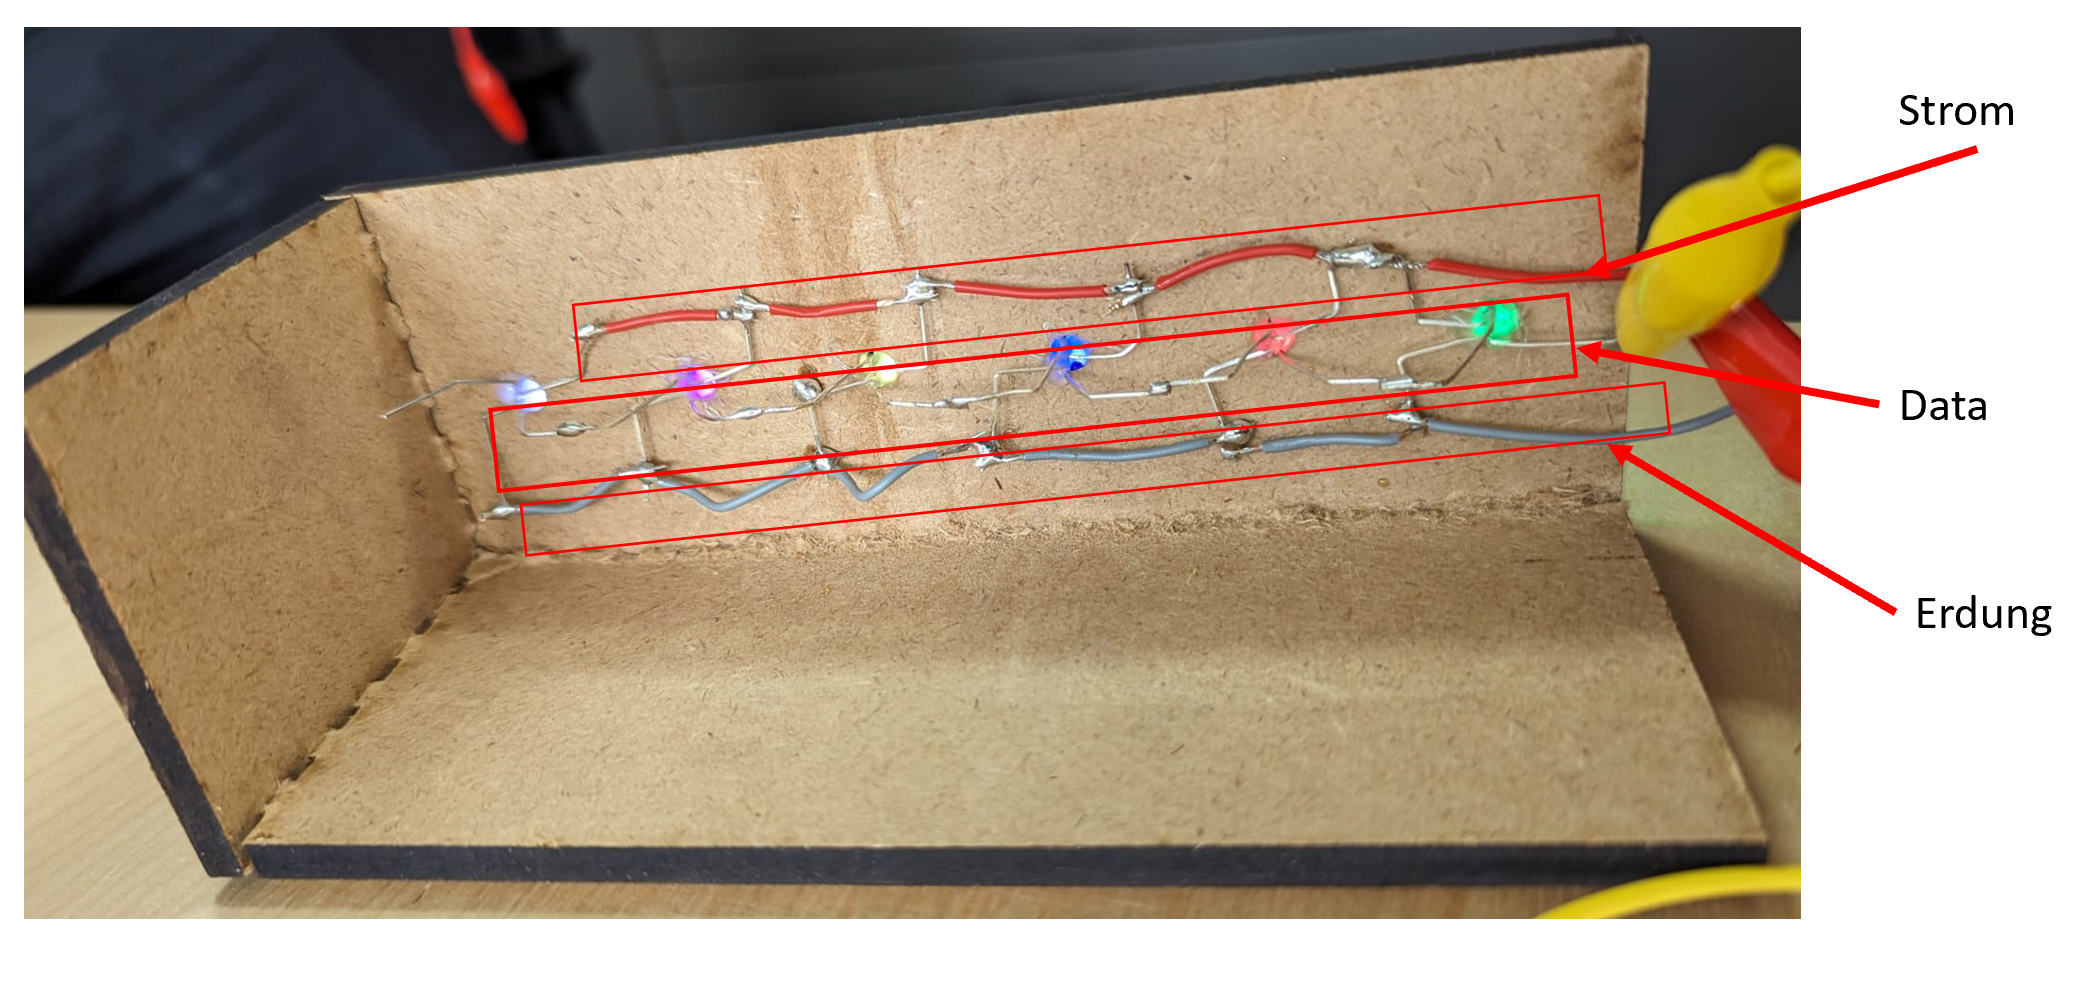
\includegraphics[width=.85\textwidth,scale=1]{./images/herzen_leds.png}}
 \caption{Zusammenlöten der LEDs}\label{herzen}
\end{figure} 

Mit dem erfolgreichen Aufbau der Prototypen und der Implementierung des finalen Gerüsts ist eine solide Basis für das spannende Spielerlebnis von Wire \& Warriors geschaffen worden.
  \chapter{Software Umsetzung}

Das Projekt stellte für uns nicht nur in Bezug auf die Hardware hohe Anforderungen, sondern erforderte auch für ein Mikrocontroller-Projekt eine ungewöhnlich komplexe Softwarelösung. Von Beginn an war es daher essenziell, eine klare und gut organisierte Struktur zu etablieren. Diese Vorgehensweise gewährleistet, dass der Code sowohl wartbar als auch übersichtlich bleibt, was für die effiziente Entwicklung des Projekts von großer Bedeutung ist.

Des Weiteren wurde von Beginn an besonderer Wert darauf gelegt, den Code unter Versionskontrolle zu stellen, wofür Git gewählt wurde. Dieser Schritt gewährleistete eine effiziente Verwaltung der Code-Änderungen und bot eine robuste Plattform für die Zusammenarbeit im Team an.

\section{Entwicklungsumgebung}

Für die Entwicklung der Software wurde Visual Studio Code (VSCode) als integrierte Entwicklungsumgebung (IDE) ausgewählt. VSCode ist aufgrund seiner vielseitigen Fähigkeiten hervorragend für die Programmierung von Mikrocontrollern geeignet. Diese Plattform zeichnet sich durch eine Vielzahl an Erweiterungen (Plugins) aus, die speziell für verschiedene Programmiersprachen und Projektspezifikationen konzipiert sind. Diese Flexibilität und Anpassungsfähigkeit von VSCode macht es zu einem idealen Werkzeug auch für dieses Entwicklungsprojekt.

\section{Programmiersprache}

Aufgrund der Nutzung des Arduino Uno als Mikrocontroller fiel die Wahl für die Entwicklungssprache auf C++. Arduino zeichnet sich durch seine umfangreichen Bibliotheken aus, die die Integration von Funktionen und Komponenten erheblich erleichtern. Diese Bibliotheken bieten eine reiche Auswahl an vorgefertigten Codes und Modulen, die es ermöglichen, komplexe Funktionen mit geringerem Aufwand zu implementieren und somit die Entwicklungszeit zu verkürzen. 

\section{PlatformIO}

Wie bereits erwähnt, zeichnet sich Visual Studio Code durch seine umfangreiche Plugin-Unterstützung aus. Für dieses Projekt wurde speziell das Plugin PlatformIO verwendet, das sich als äußerst nützlich für die Arbeit mit Mikrocontrollern erwiesen hat. PlatformIO bietet umfassende Unterstützung bei der Handhabung des Arduino Uno. Es ermöglicht nicht nur das Kompilieren des Codes, sondern auch das bequeme Übertragen auf den Mikrocontroller. Zudem bietet es die Möglichkeit, verschiedene Ausgaben über den Serial Monitor zu überwachen.

Ein zentrales Element von PlatformIO ist die 'platformio.ini'-Datei. In dieser Konfigurationsdatei werden wichtige Projektinformationen festgelegt, wie zum Beispiel der verwendete Mikrocontroller-Typ (Arduino Uno), das Framework (Arduino) und die eingebundenen Bibliotheken.

\begin{figure}[H]
    \centerline{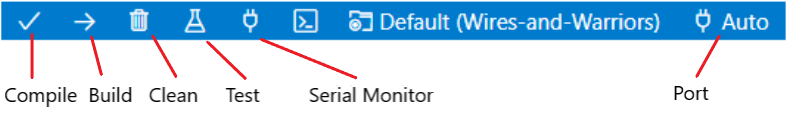
\includegraphics[width=.85\textwidth,scale=1]{./images/platformio.png}}
    \caption{PlatformIO Unterstützung in VSCode}\label{herzen}
\end{figure}

\section{Komponenten}

Bei der Entwicklung wurde ein besonderes Augenmerk einen fein gegliederten und modularen Codeaufbau gelegt. Um diesen modularen Ansatz zu unterstützen, wurde für jede Komponente (repräsentiert durch eine .cpp-Datei) eine zugehörige Header-Datei (.h) erstellt. In diesen Header-Dateien sind alle nach außen sichtbaren Methoden und Variablen der jeweiligen Komponente definiert. Dies fördert eine klare Trennung zwischen der Implementierung und der Schnittstellendefinition, was die Lesbarkeit und Wartbarkeit des Codes wesentlich verbessert.

Die Applikation wurde in folgende Hauptkomponenten unterteilt: 

\subsection{main}

Die main.cpp dient als zentrale Datei der Applikation. Ihre Hauptfunktion besteht darin, verschiedene Services und Module zu initialisieren. Zusätzlich beinhaltet die main.cpp spezifische Funktionen für Arduino, wie:

\begin{minipage}{\linewidth}
\begin{lstlisting}
void setup() { ... }
void loop() { ... }
\end{lstlisting}
\end{minipage}

\subsection{Game}

Die Game-Komponente stellt den umfassendsten Teil der gesamten Applikation dar. Sie beinhaltet die vollständige Logik, die den Zustand (State) und den Ablauf des Spiels bestimmt.

In jedem Zyklus (Tick) des Spiels wird die dazugehörige Funktion der Komponente aufgerufen. Diese Funktion übernimmt essentielle Aufgaben wie die korrekte Steuerung der LED-Anzeigen oder das Auslösen von Bewegungen der Motoren. Zusätzlich dazu beinhaltet die Game-Komponente wichtige Funktionen, die das Level-System des Spiels betreffen, wie beispielsweise die Fortschrittsverwaltung oder die Schwierigkeitssteigerung.

Hier ein vereinfachter Überblick über die Hauptfunktion dieser Komponente:

\begin{minipage}{\linewidth}
\begin{lstlisting}
// simplified version
void tick() {
    showHeartLights();

    if (checkWireTouch()) { ... }
    
    if (gameStarted) {
        turnBridge();
    }
}
\end{lstlisting}
\end{minipage}

\subsection{gameConstants}

Diese Komponente beinhaltet eine Sammlung von Konstanten, die sowohl für das Design des Spiels als auch für dessen Dynamik von entscheidender Bedeutung sind. Diese Konstanten umfassen sowohl feste Parameter, die das grundlegende Erscheinungsbild und Verhalten des Spiels definieren, als auch variierbare Elemente, die es ermöglichen, den Spielfluss sowie visuelle und auditive Effekte anzupassen. Die Flexibilität dieser Konstanten ermöglicht es den Entwicklern, mit verschiedenen Spielaspekten zu experimentieren und das Spielerlebnis zu optimieren.

Nachfolgend finden Sie einen nicht vollständigen Auszug aus dieser Sektion:

\begin{minipage}{\linewidth}
\begin{lstlisting}
// fixed values
const int lifeLEDsCount = 6;
const int pulsesForFullRotation = 6400; // motor specific

// variable values
const int errorCooldown = 1000; // milliseconds
const int volume = 25; // 0-30
\end{lstlisting}
\end{minipage}

\subsection{lights}

Die lights-Komponente ist für die Kontrolle sämtlicher Beleuchtungselemente im Spiel zuständig. Ein wesentlicher Bestandteil dieser Komponente sind die Start- und End-LEDs, welche als feste grüne LEDs an den Türmen integriert sind.

Das zweite zentrale Element der lights-Komponente sind die LEDs für die Darstellung der Herzen. Diese sind als smarte LEDs konzipiert, was bedeutet, dass sie in der Lage sind, verschiedene Farben anzunehmen. Die Farbänderungen erfolgen entsprechend dem aktuellen Zustand (State) im Spielverlauf. 

Für die Ansteuerung der Herzen-LEDs wird die Adafruit\_NeoPixel-Bibliothek verwendet. Diese Bibliothek bietet eine umfangreiche Palette an Funktionen für die Kontrolle von RGB-LEDs.

Einige der Funktionen der lights-Komponente umfassen:

\begin{minipage}{\linewidth}
\begin{lstlisting}
void showGameNotStarted() { ... }
void showHearts(int playerHeartCount) { ... }
void showError(int lastError) { ... }
void showRingLights() { ... }
\end{lstlisting}
\end{minipage}    

\subsection{logging}

Die Logging-Komponente ist ausschließlich für Debugging-Zwecke konzipiert. Ihr Hauptmerkmal ist eine globale Log-Funktion, die für die Protokollierung von Informationen während der Entwicklungs- und Testphasen des Spiels verwendet wird. Diese Funktion nutzt den Standardmechanismus des Serial Monitors, um Log-Nachrichten auszugeben, mit dem einzigen Unterschied, dass eine Überprüfung stattfindet, ob die Logging-Funktion aktiviert ist, bevor irgendwelche Nachrichten protokolliert werden.

\subsection{motor}

Die motor-Komponente ist zuständig für die Steuerung aller Motoren im Spiel. Sie umfasst sowohl die Kontrolle des Motors für das Brückenelement als auch die Ansteuerung der Motoren, welche die Drähte an den Türmen bewegen.

Außerdem ein wichtiger Bestandteil dieser Komponente sind die Überprüfungsfunktionen, die kontrollieren, ob und wann eine Drehung der Motoren durchgeführt werden soll. Details dazu werden später genauer erläutert.

Als Beispiel für die Funktionalität dieser Komponente dient die Funktion zum Drehen der Turmdrähte:

\begin{minipage}{\linewidth}
\begin{lstlisting}
void turnSides(int level) {
    if (!timeToTurnSides()) {
        return;
    }

    for (int i = 0; i < getMotorRotations(level); i++) {
        // turn side motors one step
        digitalWrite(stepPinWire, HIGH);
        delayMicroseconds(1); // we need the delay
        digitalWrite(stepPinWire, LOW);
    }
}
\end{lstlisting}
\end{minipage}  


\subsection{pins}
Die pins-Datei spielt eine wesentliche Rolle in der Organisation und Konfiguration des Projekts, indem sie eine klare und strukturierte Übersicht über die Belegung aller Pins bietet. In dieser Datei werden alle Pins, die für die Verbindung des Arduino-Boards mit den verschiedenen Komponenten des Systems verwendet werden, über Konstanten definiert.

Diese systematische Zuordnung ist besonders hilfreich während der Verkabelungsphase, da sie eine genaue und fehlerfreie Verbindung der Hardware-Komponenten mit den entsprechenden Pins des Arduino-Boards gewährleistet. Änderungen in der Hardware-Konfiguration können somit leichter umgesetzt werden, indem die entsprechenden Werte in der pins-Datei angepasst werden, ohne den Hauptcode des Projekts zu beeinflussen.

\subsection{touch}
Diese Komponente ist eine unterstützende Funktionseinheit, die speziell für die Erkennung von Berührungen an bestimmten Pins konzipiert wurde. Diese Funktion ist ein kritischer Bestandteil des Spiels und wird in verschiedenen Szenarien eingesetzt, wie beispielsweise beim Start des Spiels, beim Erreichen des Ziels oder bei der Erkennung eines Fehlers, also einer Berührung des Drahtes.

Die Kernfunktion der touch-Komponente nutzt die digitalRead()-Funktion, die von der Arduino-Bibliothek bereitgestellt wird.

\begin{minipage}{\linewidth}
\begin{lstlisting}
bool playerTouchesPin(int pin) {
    return !digitalRead(pin);
}
\end{lstlisting}
\end{minipage}

\section{Asynchronität der Software}

Die Herausforderung, mehrere Funktionen gleichzeitig auszuführen, war ein komplexes Problem im Rahmen dieses Projekts. Insbesondere mussten die Motoren kontinuierlich laufen, während das Spiel fortschritt, Berechnungen durchgeführt und ständig auf Berührungen geprüft wurden.
Dies stellte sich als besonders schwierig heraus, da außerdem im Spiel zahlreiche zeitbasierte Funktionen existieren, wie etwa Fehler-Cooldowns mit Animationen sowie Start- und Endanimationen für jedes Level.

Anfangs wurde versucht, das Problem mit Verzögerungen (Delays) im Code zu lösen. Diese Methode führte jedoch zu nicht nachhaltigen Lösungen und verursachte während der Entwicklung immer wieder Bugs.
Die endgültige Lösung des Problems fand sich in der Verwendung von Zeitstempeln. An verschiedenen Stellen in der Anwendung wird ein Zeitstempel gesetzt und anschließend überprüft, ob eine bestimmte Zeitspanne verstrichen ist.

Diese Methode ermöglicht es, eine Art von Asynchronität zu simulieren. Durch das Arbeiten mit Zeitstempeln statt festen Verzögerungen kann das Programm fortlaufend andere wichtige Aufgaben ausführen, während es gleichzeitig auf das Erreichen bestimmter Zeitpunkte wartet. Dieser Ansatz verbessert nicht nur die Ansprechbarkeit (Reaktion) des Programms, sondern erhöht auch die Stabilität und Zuverlässigkeit des Codes, indem er die typischen Probleme vermeidet, die mit der Verwendung von Delays einhergehen.

\subsection{Beispiel}

Dieses Vorgehen lässt sich gut am Beispiel der Funktionalität zum Drehen des Brückenmotors illustrieren. Die turnBridge()-Funktion beginnt mit einer Überprüfung, ob eine Drehung der Brücke überhaupt möglich ist. Diese Überprüfung wird durch die Funktion timeToTurnBridge() realisiert, die auf Zeitsteuerung basiert. Es wird kontrolliert, ob die festgelegte Zeitspanne seit dem letzten Aktivieren der Brückendrehung verstrichen ist. Sobald festgestellt wird, dass die definierte Zeitspanne abgelaufen ist, wird der Brückenmotor aktiviert und der Zeitstempel aktualisiert, um den nächsten Zeitpunkt für eine mögliche Aktivierung zu markieren.

\begin{minipage}{\linewidth}
\begin{lstlisting}
// vereinfachte version
void turnBridge() {
    if (!timeToTurnBridge()) {
        return;
    }
    
    ...
}

bool timeToTurnBridge() {
    bool timeToTurn = elapsedTime >= motorDelay;

    if (timeToTurn) {
        lastBridgeTurnTime = currentTime;
    }

    return timeToTurn;
}
\end{lstlisting}
\end{minipage}
  \chapter{Ausblick und Fazit}

\section{Ausblick}

Das aktuelle Design des Spiels ist im Großen und Ganzen gut durchdacht und funktioniert einwandfrei. Jedoch haben wir eine Schwachstelle identifiziert, und zwar im Bereich des Brückensegments. Dieses Element ist essentiell für das Spiel, da es den Spielern ermöglicht, einander zu passieren und zur gegenüberliegenden Seite zu gelangen. Gleichzeitig stellt es jedoch einen kritischen Punkt dar, an dem die Fairness der Spieler gefordert ist. Theoretisch könnten Spieler diese Stelle nutzen, um aus dem vorgegebenen System auszubrechen und das Spiel auf eine unfaire Weise zu beenden.

Wir haben verschiedene Entwürfe und Konzepte für einen Tunnel erarbeitet, der das Überqueren der Brücke erlaubt, ohne die Möglichkeit zu bieten, das System zu umgehen. Leider konnte keine dieser Ideen das Problem zufriedenstellend lösen. Letztendlich haben wir uns entschieden, die Situation so zu belassen, wie sie ist, und setzen auf das faire Verhalten der Spieler.

Diese Entscheidung spiegelt einen Kompromiss wider, der oft in der Spielentwicklung gemacht werden muss, zwischen idealer Designlösung und praktischer Umsetzbarkeit. Wenn in Zukunft an dem Spiel weitergearbeitet wird, bietet die Lösung dieses Problems eine sinnvolle Zielsetzung.

Eine Überarbeitung des Designs könnte außerdem eine wertvolle Verbesserung für das Spiel darstellen. Die derzeitige Konstruktion aus dünnen Holzplatten, welche zusammengesteckt und teilweise mit Heißkleber und Flachwinkeln verstärkt wurden, bietet zwar die grundlegende Funktionalität, jedoch gibt es sowohl in Bezug auf Stabilität als auch auf Ästhetik Raum für Verbesserungen.

Eine einfache und kosteneffiziente Möglichkeit wäre das Färben oder Lackieren der Holzplatten. Dies würde nicht nur das ästhetische Erscheinungsbild verbessern, sondern könnte auch die Haltbarkeit des Holzes erhöhen. Verschiedene Farben oder Lackierungen könnten auch dazu beitragen, verschiedene Spielbereiche visuell zu unterscheiden. Eine umfassendere Überarbeitung könnte den Ersatz der Holzplatten durch stabilere und langlebigere Materialien beinhalten.

\section{Fazit}

\textbf{Es war ein anspruchsvolles, aber ungemein wertvolles Projekt!}

Die Projekte sind eigentlich für drei Personen ausgelegt, und leider haben wir schon früh im Projektverlauf einen Teamkollegen verloren, sodass wir nur noch zu zweit waren. Als Medieninformatiker war der Bereich der Hardware für uns ein völlig neues Terrain. Wir hatten kaum Erfahrung und verfügten über wenig Vorwissen, insbesondere in grundlegenden Aspekten der Elektrotechnik. Zwar hatten wir im Studium Module wie 'Grundlagen digitaler Systeme' oder 'Mobile and Ubiquitous Computing', doch diese sind schon einige Zeit her, und die relevanten Bereiche für dieses Projekt wurden nur teilweise abgedeckt. Da der Rest des Studiums wenig Berührungspunkte mit diesen Themen aufwies, gingen viele Kenntnisse leider wieder verloren. Daher standen wir vor der Herausforderung, uns das nötige Wissen von Grund auf anzueignen.

Besonders herausfordernd war für uns das Verständnis grundlegender Konzepte der Elektronik, insbesondere von Strom, Spannung und Widerstand. Diese Aspekte waren jedoch essentiell für das Funktionieren unseres Spiels. Glücklicherweise erhielten wir vom Team des MakerSpace wertvolle Unterstützung und Nachhilfe in diesen Bereichen, was uns enorm weiterhalf.

Ein weiteres signifikantes Problem stellte die Inbetriebnahme und Steuerung der Motoren dar, insbesondere im Zusammenhang mit den Schrittmotoren (Stepper-Motoren). Ursprünglich planten wir, kleinere Steuerungsboards einzusetzen, aber wir mussten feststellen, dass unsere Kenntnisse dafür nicht ausreichten. Schließlich entschieden wir uns für den Einsatz größerer Boards, da wir nur mit diesen eine funktionierende Lösung realisieren konnten.

Diese große Aufgabe war jedoch eine Erfahrung, die uns sehr wertvoll erscheint. Auf der Softwareseite traten glücklicherweise keine Probleme auf, was uns sehr zugute kam. Trotz der Herausforderungen und des reduzierten Teams gelang es uns, ein Projekt zu realisieren, das unsere anfänglichen Erwartungen nicht nur erfüllte, sondern in vielerlei Hinsicht sogar übertraf. Diese Erfahrung hat nicht nur unsere Fähigkeiten erweitert, sondern uns auch als Team zusammen geschweißt.
  
 
  % Literaturverzeichnis
  \phantomsection
  \addcontentsline{toc}{chapter}{Literaturverzeichnis}
  \newpage
  \bibliographystyle{apalike}
  \bibliography{pc.bib} 
  
  % Anhang
  \phantomsection
  \addcontentsline{toc}{chapter}{Abbildungsverzeichnis}
  \listoffigures
  \newpage

  \phantomsection
  \addcontentsline{toc}{chapter}{Tabellenverzeichnis}
  \listoftables
  \newpage
  
  %\include{anhang}
\end{document}  
